\documentclass[a4paper, 11pt]{article}
%\usepackage[utf8]{inputenc}
\usepackage{appendix}
\usepackage{listings}
\usepackage{color}
\usepackage{xcolor}
\usepackage{float}
\usepackage[british]{babel}
\usepackage{amsmath}
\usepackage{amsfonts}
\usepackage{amssymb}
\usepackage{amsthm}
%\usepackage{amsrefs}
\usepackage{enumerate}
\usepackage{graphicx}
\usepackage{caption}
\usepackage{subcaption}
\usepackage{url}
\usepackage[round]{natbib}
\usepackage[all]{xy}
\usepackage{tikz}
\usepackage{hyperref}
\usepackage[percent]{overpic}
\usepackage[printwatermark]{xwatermark}
\usepackage{epstopdf}
\usepackage{fancyvrb}
\usepackage{longtable}
\usepackage{wasysym}
%\usepackage{multicol}
\usepackage{pgfplots}
%\usepackage{newtxtext,newtxmath}
%\newwatermark[allpages,color=red!20,angle=45,scale=4,xpos=0,ypos=0]{DRAFT}

%\usepackage{antpolt}
%\usepackage[T1]{fontenc}
%\usepackage{tocloft}
\usepackage{selinput}
\SelectInputMappings{
  adieresis={ä},
  edieresis={ë},
  idieresis={ï},
  udieresis={ü},
  eacute={é},
}

\newcommand{\widefigwidth}{\textwidth}
\newcommand{\mgraphheight}{.21\textheight}

\usetikzlibrary{positioning}

\definecolor{MidnightBlue}{RGB}{11,28,121}
\definecolor{dkgreen}{rgb}{0,0.6,0}
\definecolor{mauve}{rgb}{0.58,0,0.82}

\newcommand{\citeneed}{{\color{red} [citation needed] }}
\newcommand{\citepos}{{\color{orange} [citation needed?] }}
\newcommand{\todo}[1]{{\color{red} TODO:} {\color{dkgreen} #1}}
\newcommand{\ennl}[1]{{\color{red} \it [TL: #1]}}

\newcommand{\Python}{\texttt{Python}}

\renewcommand{\thefigure}{\arabic{section}.\arabic{figure}}

\newcommand{\mat}[1]{\left(\begin{matrix} #1 \end{matrix} \right)}
\newcommand{\HRule}{\rule{\linewidth}{0.5mm}}
%\renewcommand{\cftdot}{}
%\renewcommand{\cftsecleader}{\cftdotfill{\cftdotsep}}
\setcounter{tocdepth}{3}

\usepackage{tikz}
\usetikzlibrary{shapes,arrows}

\floatstyle{ruled}
\newfloat{example}{htb}{lop}
\floatname{example}{Example}
\newfloat{codeblok}{htb}{lop}
\floatname{codeblok}{Codeblok}

%\newcommand{\citep}[1]{\cite{#1}}\newcommand{\citet}[1]{\cite{#1}}
\renewcommand{\cite}[1]{\citep{#1}}

\renewcommand{\lstlistingname}{Codeblok}
\lstdefinestyle{lstjava}{
language=Java,
numbers=left,
numberstyle=\tiny\color{red},
stepnumber=5,
numbersep=5pt,
tabsize=2,
breaklines=true,
keywordstyle=\color{MidnightBlue},
commentstyle=\color{dkgreen},
stringstyle=\color{mauve},
morekeywords={}
}
\lstdefinestyle{lstmatlab}{
language=Matlab,
numbers=left,
numberstyle=\tiny\color{red},
stepnumber=5,
numbersep=5pt,
tabsize=2,
breaklines=true,
keywordstyle=\color{MidnightBlue},
commentstyle=\color{dkgreen},
stringstyle=\color{mauve},
morekeywords={linreg,linregquad,logreg,ones,repmat}
}
\lstnewenvironment{lstmat}{
\lstset{style=lstmatlab}}{}

\lstnewenvironment{lstsource}{
\lstset{
language=C,
breaklines=true,
showspaces=false,
showstringspaces=false,
showtabs=false,
morekeywords={}
}}{}

\lstdefinestyle{lstcpp}{
language=C++,
numbers=left,
numberstyle=\tiny\color{red},
stepnumber=5,
numbersep=5pt,
tabsize=2,
breaklines=true,
keywordstyle=\color{MidnightBlue},
commentstyle=\color{dkgreen},
stringstyle=\color{mauve},
morekeywords={}
}

\newsavebox\mybox
\savebox\mybox{\tikz[color=red,opacity=0.1]\node{DRAFT};}
%\newwatermark*[allpages,angle=45,scale=10,xpos=-20,ypos=15]{\usebox\mybox}
\title{Detecting Plastic Soup automatically}
\author{Student:\\Ysbrand Galama \\ Stud.ID: 10262067 \and Supervisor:\\ Thomas Mensink }
\date{\today}

%\begin{figure}[h!tb]
%\centering
%\ifx\showfig\undefined
%\includegraphics[keepaspectratio=true,width=.6\textwidth]{images/}
%\fi
%\caption{}
%\label{fig:}
%\end{figure}

%\begin{table}[h!tb]
%\centering
%\caption{}
%\label{tab:}
%\begin{tabular}{ccc}
%1&1&1
%\end{tabular}
%\end{table}

\begin{document}
%\def\showfig{1} %-- comment to show figures
%\def\showapp{1} %-- comment to show appendix
%\def\showintro{1} %-- comment to show titlepage
%\def\showpbreak{1} %-- comment to flush pages
%\def\showmixi{1} %-- comment to show train-test above-below
%\pagenumbering{gobble}

\ifx\showintro\undefined
\begin{titlepage}
\begin{center}

\includegraphics[width=0.9\textwidth]{images/uva-campus.pdf}\\[0.5cm]


\textsc{\large Bachelor Opleiding Kunstmatige Intelligentie}\\[1cm]

\HRule \\[0.4cm]
{\bfseries { \huge Detecting Plastic Soup automatically
} \\[0.2cm]
{\it \Large  Using pre-trained Convolutional Neural Networks and Support Vector Machines}
\\[0.4cm] }

\HRule \\[1cm]

Bachelor thesis\\
Credits: 18EC\\[0.5cm]
University of Amsterdam\\
Faculty of Science\\
Science Park 904\\
1098 XH Amsterdam\\[0.5cm]

\vfill

% Author and supervisor
\begin{minipage}[t]{0.4\textwidth}
\begin{flushleft}
\emph{Author:}\\
Ysbrand M. A. A. \textsc{Galama}\\
\small UvAID: 10262067
\end{flushleft}
\end{minipage}
\begin{minipage}[t]{0.5\textwidth}
\begin{flushright}
\emph{Supervisor:} \\
Thomas \textsc{Mensink}\\[0.4cm]
\small Intelligent Sensory Information Systems\\
%Faculty of Science\\
University of Amsterdam\\
%Science Park 904\\
%1098 XH Amsterdam\\
\end{flushright}
\end{minipage}
\vfill

% Bottom of the page
{\large \today}

\end{center}
\end{titlepage}
\thispagestyle{empty}
$\,$
\vfill
\begin{abstract}
Large amounts of plastic end up in the world's oceans.
This project uses state-of-the-art Computer Vision techniques to detect Plastic Soup.
Recent studies have shown that Convolutional Neural Networks (CNN) can classify images within the classes the network was trained on with high accuracy.
While this project did not train a CNN, a CNN was used as a feature extractor for a Support Vector Machine (SVM).
The goal of this project was to develop a system based on state-of-the-art techniques that is able to distinguish plastic and animals in images.
The tests conducted in this project show a high accuracy on the dataset that was constructed for this project, making it possible to detect images containing floating plastic.
The resulting pipeline was able to classify images containing plastic and animals.
There were even several test resulting in the localisation of Plastic Soup within the images, however more research is needed before this can be used as a real-world application.
%This is the abstract... Lorem ipsum dolor sit amet, consectetur adipiscing elit. Mauris placerat erat vitae semper fringilla. Integer rhoncus sed libero quis hendrerit. Duis et nunc convallis, porttitor urna quis, ultrices nunc. Ut quis ornare neque. Vivamus rutrum nunc arcu, ac pretium nulla lobortis ac. Duis a lectus ex. Fusce eget nulla at metus commodo posuere. Proin et velit sed augue interdum lobortis. Mauris ut nisi suscipit purus dictum rutrum vitae non erat. Nulla non semper turpis, nec eleifend mi. Proin ut bibendum est, quis auctor ante.
\end{abstract}
\vfill
\vfill
$\,$
\newpage
\tableofcontents
\newpage
\else
\noindent {\it NOTE to reader: this section is not yet finished, therefore several comments are written between the sentences which can be ignored.}\\ \mbox{}~\hfill{Ysbrand Galama, \today}
\fi

\section{Introduction}
\label{sec:Introduction}
%wat, waar, waarom
%maatschappelijke bijdrage van het project
The environment is constantly being influenced by humanity and this influence has been debated since the hippie movement in the '60s.
The debate whether humanity puts too much pressure on the environment has only increased in recent years; the full impact of oil-spills and climate change are still being discussed.

This project will focus on an environmental hazards that has recently become apparent: Plastic Soup.
However, the project will not focus on how Plastic Soup affects nature, but how Artificial Intelligence can help to clean up the waste.

%Environment is important, AI can help with the conservation... [oa citeren van \citep{vannature}]


\subsection{Plastic Soup: An environmental problem}
\label{sec:Intro-Plastic Soup}
%Bede context, Maatschappelijke relevantie
%Large amounts of plastic waste ends up in the world's ocean... [oa citeren van \citep{barnes2005drifting}, \citep{moore2011plastic}]
Large amounts of plastic waste end up in the world's oceans and have a significant impact on marine life \citep{barnes2005drifting}.
Plastic Soup or Plastic Ocean are both collective nouns for this environmental problem.
As \citeauthor{barnes2005drifting} indicate, the amount of flotsam in the oceans increases annually as does the increasing proportion of plastic.

When people dispose plastic objects not in trash cans, but near rivers, wind and water flow ensure the objects float through rivers into the ocean.
The currents in the oceans transport the flotsam around the oceans where it settles in patches.
In figure \ref{fig:plastic-where} the estimated location of the Great Pacific Ocean Patch is shown.
Plastic does not decay in nature, therefore a sizeable portion of marine life ingests the plastic after which it ends up in their digestive system. 
Figure \ref{fig:plastic-bird} shows how much plastic can end up in a bird.
In addition to the dangers for marine life, large amounts of plastic end up on beaches, as shown in figure \ref{fig:plastic-beach}.
This has a sizeable impact on local society and economy.

\begin{figure}%[h!bt]
  \centerline{
   \begin{minipage}{\widefigwidth}
 	\begin{center}
     \begin{subfigure}[t]{.65\textwidth}
      \ifx\showfig\undefined
       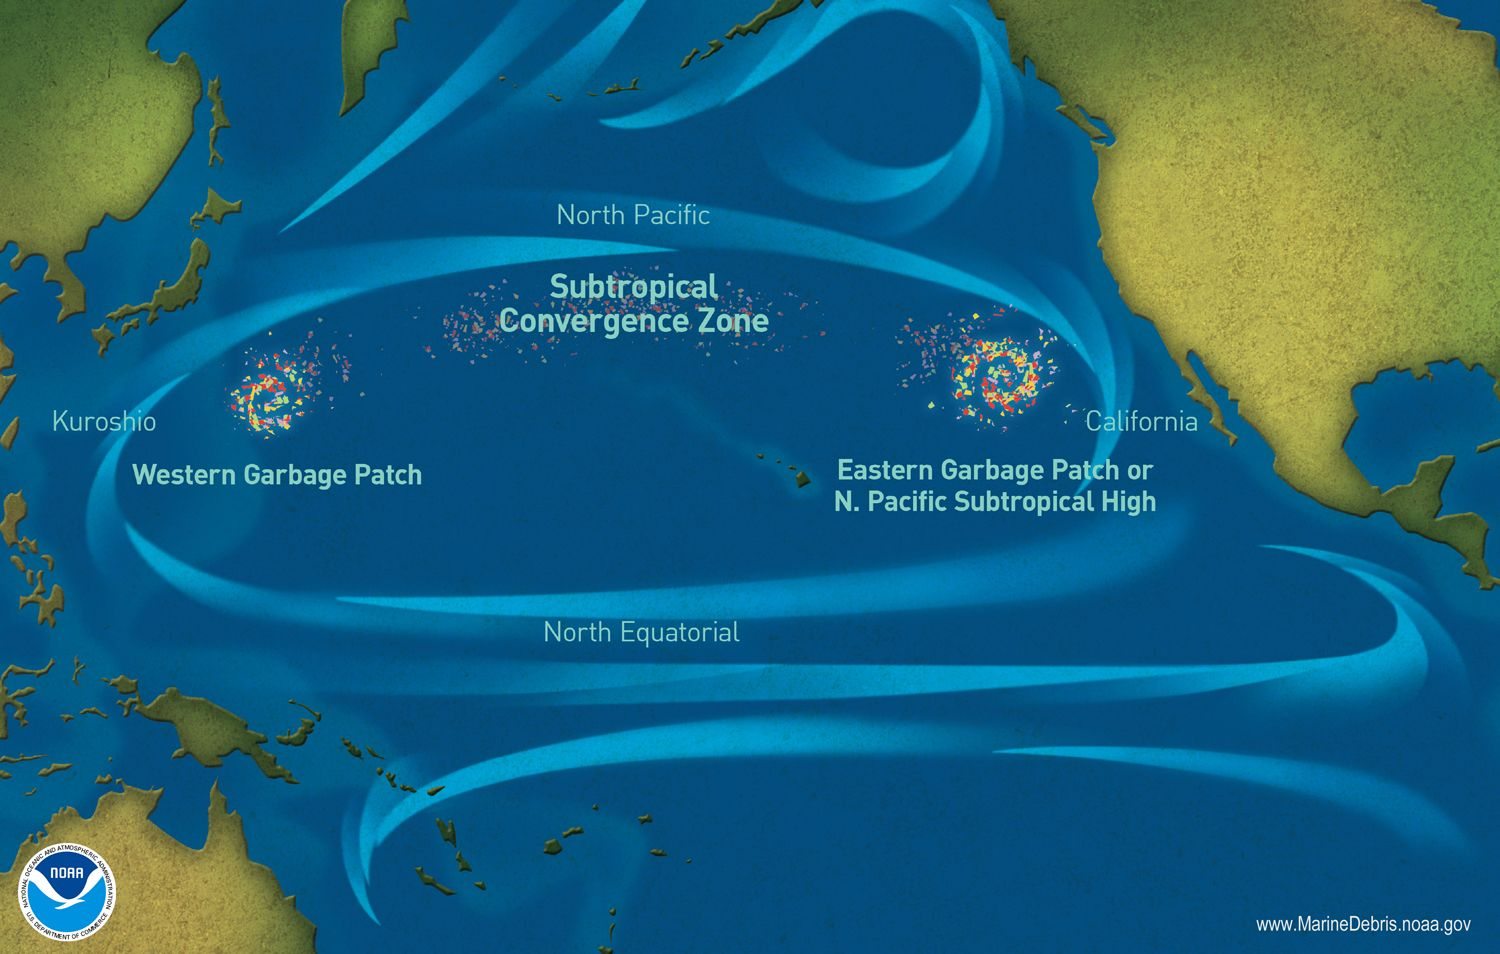
\includegraphics[keepaspectratio=true,width=\textwidth]{images/garbage-patch.jpg} \fi
      \caption{Ocean currents in the Pacific that `collect' the Plastic Soup. Map by NOAA source: \url{http://education.nationalgeographic.com/education/encyclopedia/great-pacific-garbage-patch}}
      \label{fig:plastic-where}
     \end{subfigure}
    \end{center}\\
   \begin{subfigure}[t]{.48\textwidth}
    \ifx\showfig\undefined
	 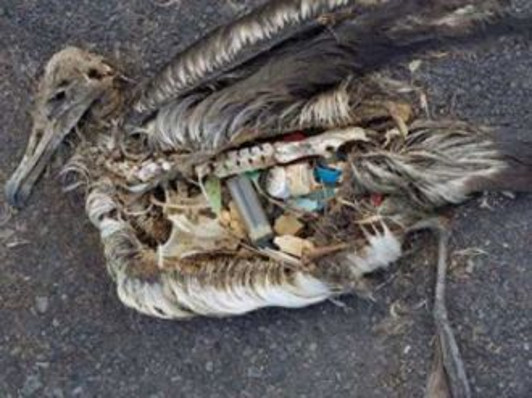
\includegraphics[keepaspectratio=true,width=\textwidth]{images/Bird_with_plastic_stomach.jpg} \fi
	\caption{The stomach contents of a bird that ate plastic. Photograph by Chris Jordan, U.S. Fish and Wildlife Service }
	\label{fig:plastic-bird}
   \end{subfigure}
   \hfill
   \begin{subfigure}[t]{.48\textwidth}
    \ifx\showfig\undefined
	 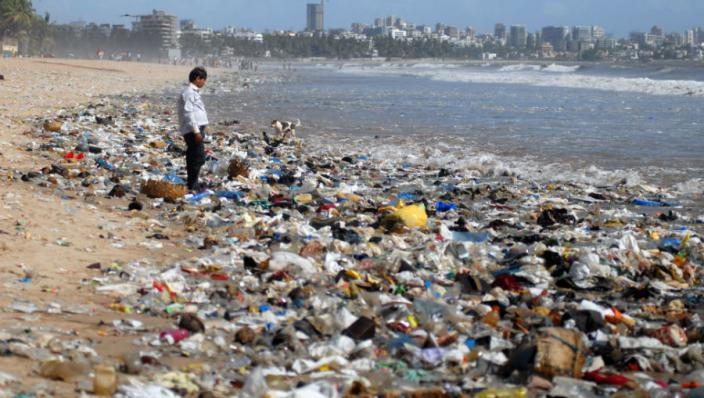
\includegraphics[keepaspectratio=true,width=\textwidth]{images/plastic-beach.jpg} \fi
	\caption{A polluted beach in Mumbai, India. Photograph by EPA }
	\label{fig:plastic-beach}
   \end{subfigure}
   \caption{Three images that show the impact of Plastic Soup on the environment and society.}% (a) shows where the sea-currents deposit the plastic. (b) shows how much plastic can end up in a bird. (c) shows a polluted beach in Mumbai, India.}
   \label{fig:plastic-impact}
   \end{minipage}
  }
\end{figure}

The most significant problem is probably micro-plastic.
When plastic floats in water for some time, sunlight and minerals break the plastic objects down into grains.
These grains of plastic are usually only several micro meters in size and can infect the ecosystem to a large extend \citep{moore2011plastic}.
The full impact of micro-plastic is still unknown, however these plastic grains can end up in bloodstreams of animals and even humans and clog their arteries.

To recapitulate, Plastic Soup can influence the environment to a large extend.
The oceans become polluted with plastic and it kills marine life. Above that society is also influenced and it is even possible that humans die from ingesting micro-plastic.

The pressure of Plastic Soup on the environment has caused several organisations to form in order to address this problem and find solutions for the problem.
The nascency of organisations addressing this problem and searching for solutions have gained media attention and thus cause the growing awareness for the Plastic Soup.
These organisations would benefit of systems that can detect plastic automatically.
Therefore, this project will focus on techniques that are able to distinguish plastic from marine life in ocean water.
The goal of this project is to develop a system based on state-of-the-art techniques that is able to distinguish plastic from animals in images.

\subsection{Project outline}
\label{sec:Intro-Me}
%Onderzoeksvraag, proefopzet, hypothese
To develop a system that can detect plastic, state-of-the-art imaging techniques will be used.
In recent years the accuracy of imaging techniques on object recognition have steadily increased, as section \ref{sec:Theory} describes.
This project will research how these techniques will perform on Plastic Soup detection.

A dataset of annotated images will be constructed to be used in this project.
This dataset can be used to train and test the build system.
To recognise the images containing plastic, a Convolutional Neural Network (CNN) will be used.
The CNN will not be trained on the data itself but a pre-trained network will be used to construct a feature-vector of the image.
These feature-vectors will be used to train a classifier to classify the images in either containing plastic or not containing plastic.
The classifier used in this project is a Support Vector Machine (SVM); to distinguish between plastic and marine-life, two SMVs will be trained.

Both CNNs and SVMs are known to reach high accuracy in Computer Vision, therefore it is hypothesised that this method for plastic recognition should give an appropriate baseline.

Besides the detection of images containing plastic, this project will also research if the location of the plastic within an image can be detected.
As a prove of concept, the pipeline of the plastic recognition will be adapted a small amount to give results for localisation.
%To truly localise the plastic in the image, more research will be necessary.

\subsection{Outline of the thesis chapters}
\label{sec:Intro-Outline}
The performance of the plastic-soup detector created in this project are described in section \ref{sec:Conclusion} with the tables of the results located in section \ref{sec:Results}.
In section \ref{sec:Method} the method of the project is described, section \ref{sec:Data} shows how the data used in this project was acquired, and in section \ref{sec:Discussion} I will go into the parts that can be improved in further research.
But first, in section \ref{sec:Theory} the current state-of-the-art techniques in the field of Computer Vision will be discussed.
%In section \ref{sec:Theory}... \todo{when the thesis is finished, fill this paragraph}















\iffalse
%...dangers of microplastic...

%...big impact on marine life and life in general...

%==Urgentie had groter kunnen worden gemaakt. Hoeveel plastic is er? Wat wordt er al aan gedaan? Hoeveel vogels hebben er last van? Waar komt dat plastic vandaan? Etc.

\subsection{Current solutions}
\label{sec:Intro-Current}


One of the organisations that addresses the problem is Saraswater \citeneed.
This organisation is developing techniques to clean the ocean of this plastic waste.
Saraswater made an apparatus that can be mounted on a ship which shovel the waste from the water.
The small scale experiments that they performed show promising results.

These plastic shovelling ships would benefit from being autonomous.
If no humans are needed, the ships can roam the oceans for many months without the need for visiting harbours.

%One of them is Saraswater. They are developing techniques .. [oa bronnen van de organisaties (niet zozeer artikelen)]
%To help she ships of saraswater, atomise the process with autonomous agents...
%laatse zin: dit is niet genoeg, automatiseering
\subsection{Automation}
\label{sec:Intro-Automate}
When the ships are controlled by an autonomous agent, less human labour is needed for the clean up of the Plastic Ocean.
This project will try to begin with automation of the clean-up.

The automation of the ships is a long term goal.
Before the ships of Saraswater can be autonomous, they first need to `see' to know where the plastic is to clean up.
That is why this project will focus on detecting plastic in ocean water from image data.
Further research expanding this project could develop true autonomous agents controlling the plastic shovelling ships.



%Using state-of-the-art imaging techniques... probably effect... Investigate what will work best by using different algorithms on a dataset of annotated images...


\fi
%\ifx\showpbreak\undefined \clearpage \fi

\section{Theoretical framework}
\label{sec:Theory}
%Zijn er knowlage/algorithme `gaps'
%wetenschappelijke bijdrage van dit project
%\subsection{Image recognition}
%\label{sec:Theory-CV}
The history of Image Recognition begins as a summer school of Stanford.
As was the case in that age, Artificial Intelligence made some wild assumptions on the reachability of their projects. \citeneed
The recent developments show how mistaken they were.

Through the years multiple algorithms have been made to accomplice Computer Vision.
The model used to describe images has been a grid with a value (the pixels).
This results in a multidimensional function, on which several linear and geometric algebra algorithms can be used on.
Usually three steps are taken to identify an image.
First using the gradient in images, key-points of the image are identified.
Thereafter, these key-points are used to construct features or models, describing the image.
Finally these models are tested against a classifier. \citeneed

%The Convolutional Neural Network uses the same kind of steps.
%However, part of the models and representations of the images are not made by humans, as is the case in most other algorithms, but learnt by the network itself.

\subsection{Image representations}
\label{sec:Theory-image}
As stated above, local image gradients are used to make models on which classifiers can be trained.
Several techniques exists that extract features from the image and make a descriptor.
A wildly used technique for extracting the features is a `Bag of Features'; the frequency of the features result in a multidimensional vector of the size of the number of features.
From the data-points representing the images, a classifier can be trained. \citeneed

Another possibility is using a Convolutional Neural Network.
The CNN does a similar trick with the features.
However, it also constructs the features itself from the image-data and has the possibility to be used as a classifier.
In other words, a CNN can be used for each of the steps needed for classifying images.

The CNN technique is currently popular with image recognition tasks.
From large amounts of data, an accurate recognition system can be trained \citep{girshick2014rich}, \citep{razavian2014cnn}.

The biggest difference between `classical' imaging techniques --such as Bag of Features-- and Convolutional Neural Networks is the self-learning of the CNN.
The neurons of a CNN are trained on the data and construct their own representation that describes the images.
In contrary to classical techniques, from which the representations are constructed by humans that build the algorithms.

%\todo{structuur: -image representations(bow, cnn). -image classification (svm=meest voorkomend)}

%Eerdere bevindingen recognition %--/kleur
%Current image recognition and detection algorithms specialise on neural-nets... [oa citeren \citep{szeliski2010computer}] Current state-of-the-art results...
% Kriz, Hinton of LeCun was logischer geweest. Of naar de hele ImageNet 2014 competitie
%\subsection{CNN}
%\label{sec:Theory-CNN}
%What is CNN and how does it work... [oa citeren \citep{jia2014caffe}, \citep{razavian2014cnn}, \citep{girshick2014rich} ]
%...CNNs exist since the 1980's... mimic part of human brains...
%...layers of neurons... weights...
%==waarom CNNs zo goed werken lijken te voor image recognition en speech recognition tasks. 
%...since 2011 implementation for fast calculations on GPU...
%...high performance probably because of `learned' representations instead of `man-made'...

In the Machine Learning the Convolutional Neural Network (CNN) has existed for quite some time \citep{fukushima1980neocognition}.
However, due to computational complexity is was only recently that \citet{krizhevsky2012imagenet} showed an implementation to compute large CNNs.
\citeauthor{krizhevsky2012imagenet} shows how to implement a CNN on a computer's GPU that can work with the massive parallelism necessary to compute many layers of nodes.

Neural Networks consist of nodes, connected with weighted edges.
When data is presented to the input of the network, each node calculates with its input an output, which results in an output of the network.
When the output of the network is incorrect according to the label of the input, a backward calculation in the network is performed.
This calculation makes an adaptation to the weights in such a manner, that the network will output the correct label in the next run.

A CNN is a neural network that consists of several layers of nodes, with sometimes many millions of neurons.
Figure \ref{fig:cnn-alex} shows the layers of neurons the CNN used by \citeauthor{krizhevsky2012imagenet}.

\begin{figure}[h!tb]
\centering
\ifx\showfig\undefined
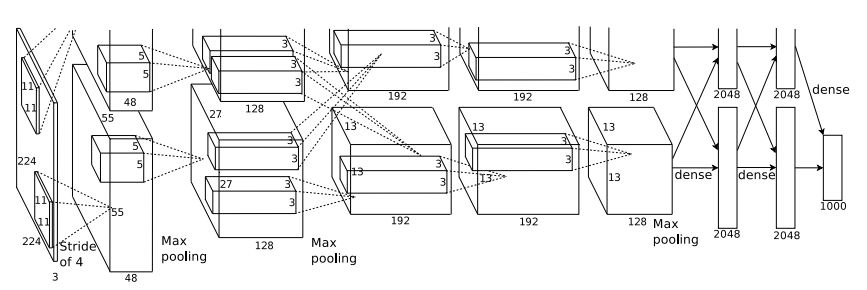
\includegraphics[keepaspectratio=true,width=\textwidth]{images/alexnet2012.png} \fi
\caption{Model of the layers of neurons in the CNN as used by \citet{krizhevsky2012imagenet}}
\label{fig:cnn-alex}
\end{figure}

Though a CNN can be used to classify a dataset of images, training such a network uses much computing power.
A pre-trained CNN has the weights of the neurons adapted to the dataset used for training.
This results in a network trained on other classes than used for this project.
However, a method that can be applied to work around this problem is inherent to the workings of a CNN.

%The dataset in this project is small with only 40k images.
%Therefore training a CNN will not be possible.
%However, because of the manner a CNN is build, it will not be necessary to fully train the network.

The bottom layers of a CNN trained on large image datasets detect basic visual concepts, for instance lines, corners and simple shapes.
Only higher in the network the concepts become more abstract and less local \citep{zeiler2014visualizing}.
Therefore, using the second-to-last layer of a pre-trained CNN an abstract representation of the image can be obtained.

This second-to-last layer can be represented as a multidimensional vector in a space the size of the number of abstract features.
As stated before, a feature-vector can be used to train a classifier.
Effectively, this project uses a pre-trained CNN as a feature extractor of an image to train an SVM classifier.

%--\subsection{Colour}
%--What is colour and why is it important... [oa citeren \citep{van2010evaluating}, \citep{ai2010color}]
%\subsection{Principal Component Analysis}
%\label{sec:Theory-PCA}
%\todo{Write this section (or delete it)}
\subsection{Image classification}
\label{sec:Theory-class}
Classifying feature-vectors has also several possible algorithms.
The Support Vector Machine (SVM) is one of the classification algorithms in Machine Learning that is wildly used in supervised image classification.
%In contrary to k-means cluster algorithm, an SVM uses labelled data to classify \citepos.
%An SVM also works better in high-dimensional data than a k-means clustering \citeneed.
%However, an SVM works best when no more than two classes need to be classified.

The SVM uses the data-points as vectors in a high dimensional space.
In this space, several Linear Algebra techniques are used to fit a hyperplane in this space, where the distance (i.e. a projection of the vector on the plane) of each data-point is maximised.
Figure \ref{fig:svm-fits} shows an example in 2D of possible manners to divide the data-points in the classes; the solid line shows a maximised classifier.
The SVM results in a classifier where the sign of the projection vector classifies the data-points (i.e. on which side of the plane the data-point is).

\begin{figure}[h!tb]
\centering
\ifx\showfig\undefined
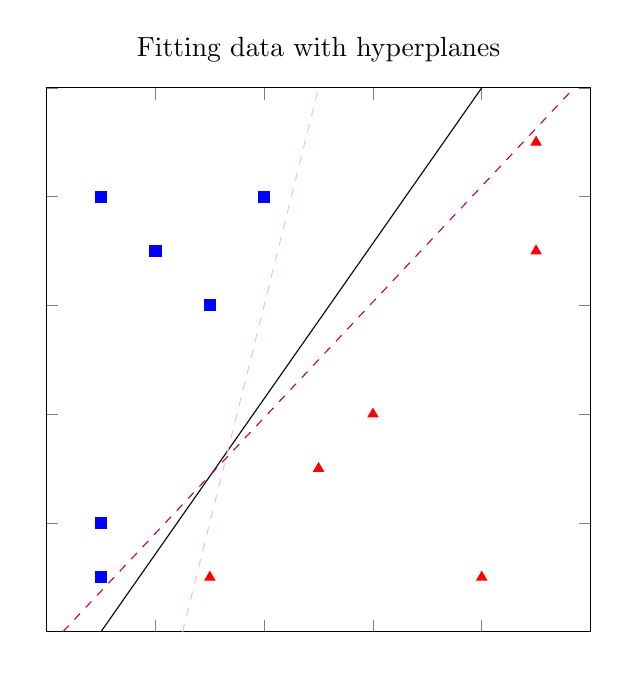
\begin{tikzpicture}
\begin{axis}[
    title={Fitting data with hyperplanes},
    width=.7\textwidth,
    height=.7\textwidth,
    xmin=0, xmax=10,
    ymin=0, ymax=10,
    yticklabels={,,},
    xticklabels={,,},
]
\addplot[
    color=blue,
    mark=square*,
    only marks,
    ]
    coordinates {
    (1,1) (1,2) (1,8) (2,7) (4,8) (3,6)
    };
\addplot[
    color=red,
    mark=triangle*,
    only marks
    ]
    coordinates {
    (3,1) (8,1) (5,3) (6,4) (9,7) (9,9)
    };
\addplot[
    color=black,
    ]
    coordinates{
    (1,0) (8,10)
    };
\addplot[
    color=pink, dashed
    ]
    coordinates{
    (2.5,0) (5,10)
    };
\addplot[
    color=purple, dashed
    ]
    coordinates{
    (0.3,0) (9.7,10)
    };
\end{axis}
\end{tikzpicture} \fi
\caption{Example of possible possible classifications in an algorithm. The dotted lines are a worse fit than the continuous one.}
\label{fig:svm-fits}
\end{figure}

The hyperplane that describes the classifier can be described by, besides linear, other, more complex, formulae.
However, these planes usually need more calculation time than a linear plane.
Figure \ref{fig:svm-planes} shows the three hyperplanes used in this project.
The data in these examples show the necessity of the different hyperplanes for different data.

\begin{figure}[h!tb]
\centering
\ifx\showfig\undefined
\centerline{
\begin{minipage}{1.3\textwidth}
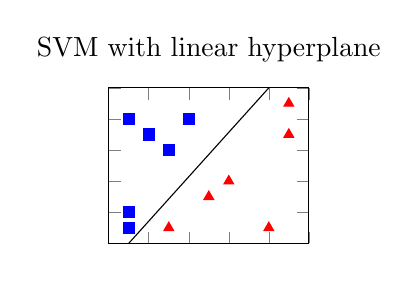
\begin{tikzpicture}
\begin{axis}[
    title={SVM with linear hyperplane},
    width=.34\textwidth,
    xmin=0, xmax=10,
    ymin=0, ymax=10,
    %xtick={0,...,10},
    yticklabels={,,},
    xticklabels={,,},
]
\addplot[
    color=blue,
    mark=square*,
    only marks,
    ]
    coordinates {
    (1,1) (1,2) (1,8) (2,7) (4,8) (3,6)
    };
\addplot[
    color=red,
    mark=triangle*,
    only marks
    ]
    coordinates {
    (3,1) (8,1) (5,3) (6,4) (9,7) (9,9)
    };
\addplot[
    color=black,
    ]
    coordinates{
    (1,0) (8,10)
    };
\end{axis}
\end{tikzpicture}
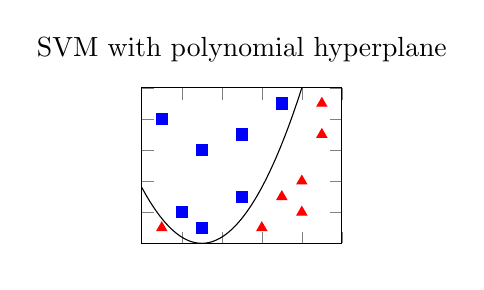
\begin{tikzpicture}
\begin{axis}[
    title={SVM with polynomial hyperplane},
    width=.34\textwidth,
    xmin=0, xmax=10,
    ymin=0, ymax=10,
    %xtick={0,...,10},
    yticklabels={,,},
    xticklabels={,,},
]
\addplot[
    color=blue,
    mark=square*,
    only marks,
    ]
    coordinates {
    (3,1) (2,2) (1,8) (5,7) (7,9) (3,6) (5,3)
    };
\addplot[
    color=red,
    mark=triangle*,
    only marks
    ]
    coordinates {
    (1,1) (6,1) (8,2) (7,3) (8,4) (9,7) (9,9)
    };
\addplot[
    color=black,
    domain=0:10,
    samples=100] (\x,{0.4*(\x-3)^2});
\end{axis}
\end{tikzpicture}
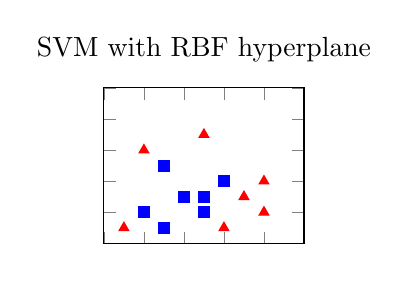
\begin{tikzpicture}
\begin{axis}[
    title={SVM with RBF hyperplane},
    width=.34\textwidth,
    xmin=0, xmax=10,
    ymin=0, ymax=10,
    %xtick={0,...,10},
    yticklabels={,,},
    xticklabels={,,},
]
\addplot[
    color=blue,
    mark=square*,
    only marks,
    ]
    coordinates {
    (3,1) (2,2) (5,2) (4,3) (6,4) (3,5) (5,3)
    };
\addplot[
    color=red,
    mark=triangle*,
    only marks
    ]
    coordinates {
    (1,1) (6,1) (8,2) (7,3) (8,4) (5,7) (2,6)
    };
\draw (axis cs:4,3) circle [black, radius=25];
\end{axis}
\end{tikzpicture}
\end{minipage}
} \fi
\caption{Examples of different hyperplanes of a two dimensional SVM }
\label{fig:svm-planes}
\end{figure}
%...classification in many dimensions... works by hyperplanes...
%--\subsection{Pre-process}
%--Before a CNN can be used, the imagedata needs to be pre-processed...
%--[oa citeren \citep{guo2010completed}, \citep{zhang2010local}]
\ifx\showpbreak\undefined \clearpage \fi
%\clearpage

\section{Dataset of Plastic Soup images}
\label{sec:Data}
Because for this project no dataset was available that consists of labelled images of floating plastic, one was constructed by hand.

The dataset used in this project was created from short films by Bill MacDonnald\footnote{The videos are online on youtube: \url{www.youtube.com/007bmac}. Thank you Bill for letting me use your films in this research}.
Several of these clips consist of floating plastic from a viewpoint both above and below water.
There were also clips that showed the presence of animals.
These clips were segmented in single frames and selected for use in this project; images that did not fall in one of the four classes (plastic, animals, both or none) were excluded.
A total of 37.165 images were left to annotate.
The annotation was done by my hand, classifying each image on viewpoint and if plastic or animals were visible.
To facilitate the annotation, a small Java-application was made.
With the use of several key-strokes, large amounts of image-data could be annotated with relative ease.
Even so, the annotation of the data took a considerable amount of time.

In total 20.635 images showed plastic only, 6.972 images showed animals only and 8.502 images show both.
The above (16.553) and below (20.612) viewpoints were separated into two datasets, to both train and test separately. 
In the above-set, a total of 14.588 images showed plastic, 6.341 images showed animals and 863 images showed neither. In the below-set, a total of 14.549 images showed plastic, 9.133 images showed animals and 193 images showed neither.
Figure \ref{fig:datasetimages} shows several examples of images in the dataset.
Both above and below water viewpoints are shown, as well as the labels the images were annotated with.

Because the images were constructed from films, many images were similar in appearance.
This fact should be taken in account when chances of overfitting occur.
%Because many images are similar in appearance, fully training a CNN will be difficult.
%CNNs usually have millions of neurons, which makes the possibility of over-fitting on this dataset present.
%Moreover using a pre-trained neural network has other advantages, which are stated in section \ref{sec:Method-Algorithm}.
%==Tweede of derde keer dat je zegt dat ‘grote hoeveelheden data’ gebruikt zijn om CNNs te trainen. Maar hoeveel dan? En is dat echt nodig? Er worden ook CNNs geleerd op MNIST (60K afbeeldingen). Waarom kan dat niet? Of ga je dat laten zien mbv een experiment?

To evaluate the results of the pipeline, the dataset was divided in a train (70\%), validate (10\%) and test (20\%) set.
Because consecutive frames were very similar, the division was done using a pseudo-random randomise algorithm which used the same seed every time.
This resulted in three sets of images that had a high distribution of the original data while consisting of the same images within each run.
This dataset made it possible to train the different algorithms used in this project and test the accuracy with the amount of labels computed correctly.

\begin{figure}%[h!tb]
\centering
\ifx\showfig\undefined
\def\iwith{.44\textwidth}
\centerline{
\begin{tabular}{rl}
\colorbox{white!0}{ \colorbox{red!70}{
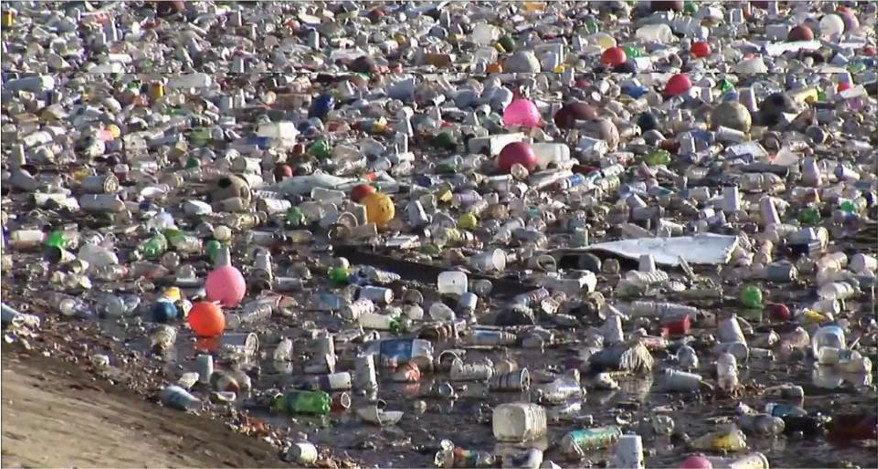
\includegraphics[keepaspectratio=true,width=\iwith]{images/matrix/253_01.jpg}}}&
%
\colorbox{white!0}{ \colorbox{red!70}{
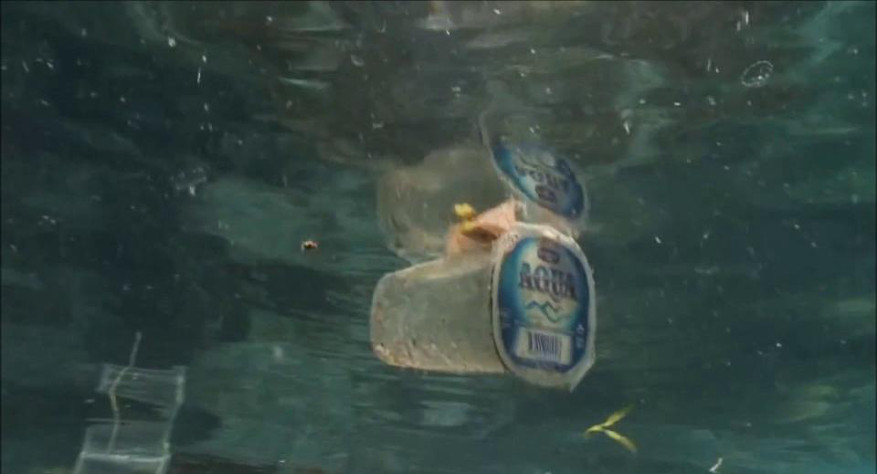
\includegraphics[keepaspectratio=true,width=\iwith]{images/matrix/20607_01.jpg}}}\\
%
\colorbox{white!0}{ \colorbox{white!0}{
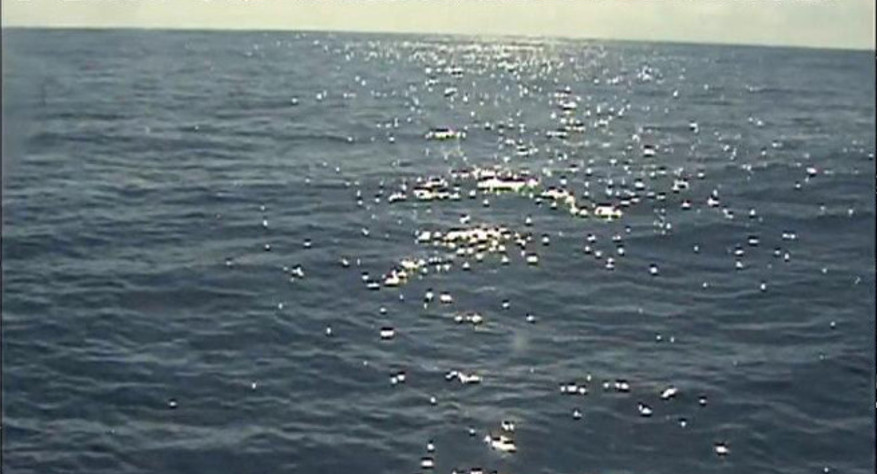
\includegraphics[keepaspectratio=true,width=\iwith]{images/matrix/299_00.jpg}}}&
%
\colorbox{white!0}{ \colorbox{green!80}{
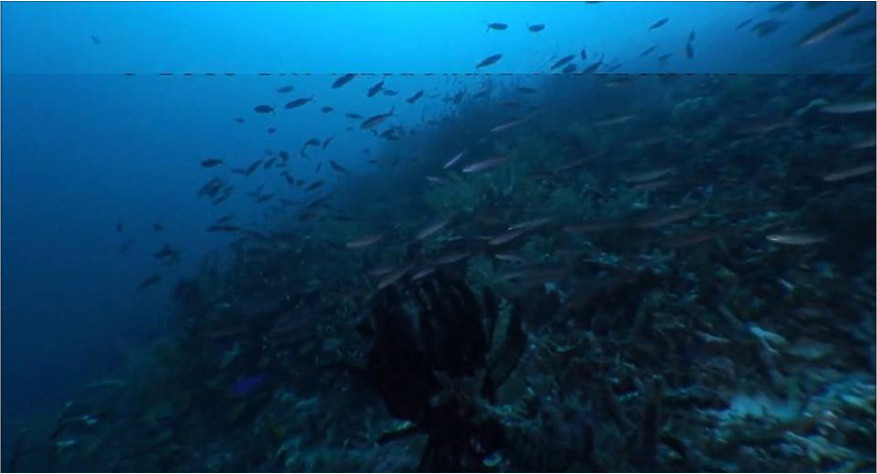
\includegraphics[keepaspectratio=true,width=\iwith]{images/matrix/2737_10.jpg}}}\\
%
\colorbox{red!70}{ \colorbox{green!80}{
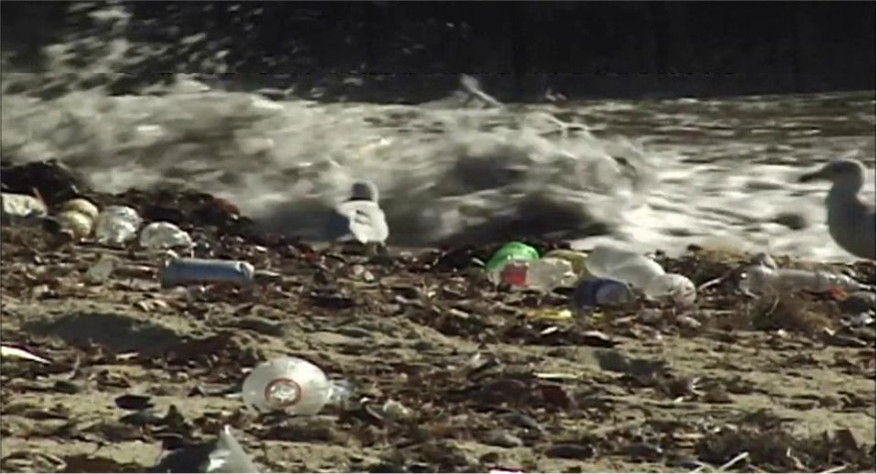
\includegraphics[keepaspectratio=true,width=\iwith]{images/matrix/31_11.jpg}}}&
%
\colorbox{white!0}{ \colorbox{red!70}{
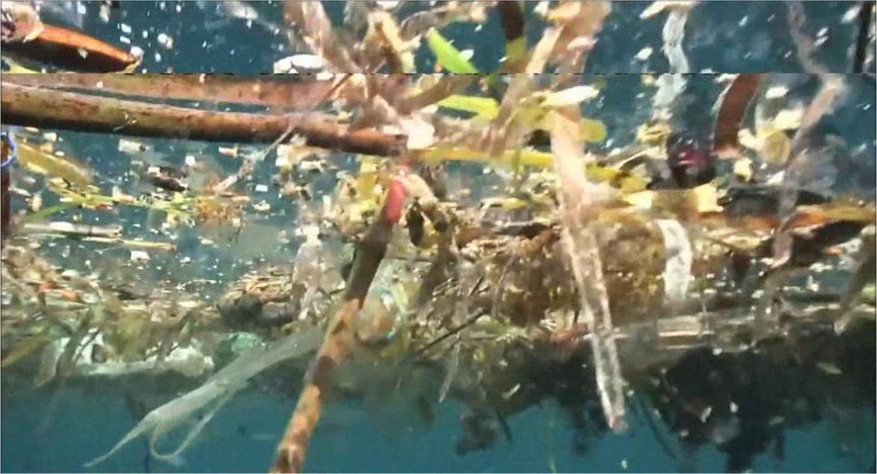
\includegraphics[keepaspectratio=true,width=\iwith]{images/matrix/4409_01.jpg}}}\\
%
\colorbox{white!0}{ \colorbox{green!80}{
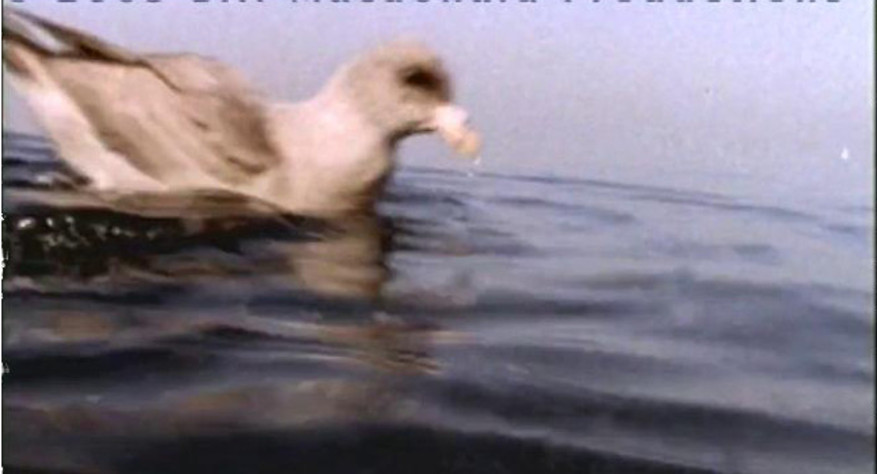
\includegraphics[keepaspectratio=true,width=\iwith]{images/matrix/401_10.jpg}}}&
%
\colorbox{white!0}{ \colorbox{green!80}{
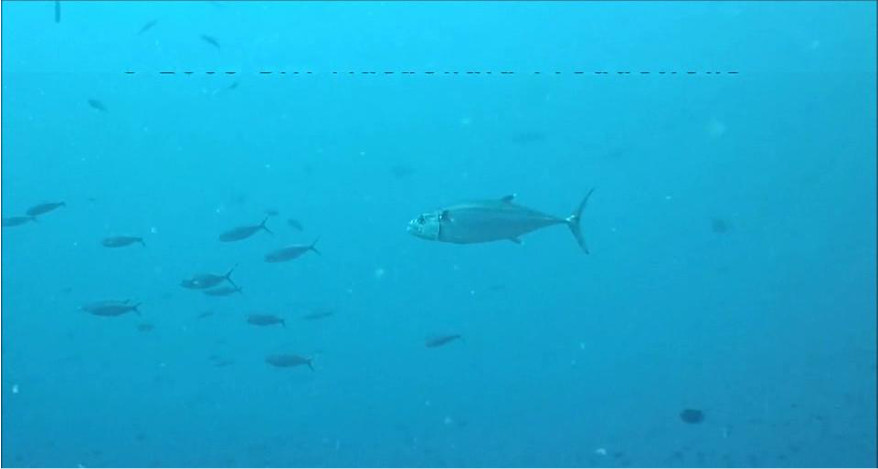
\includegraphics[keepaspectratio=true,width=\iwith]{images/matrix/5053_10.jpg}}}\\
%
\colorbox{red!70}{ \colorbox{green!80}{
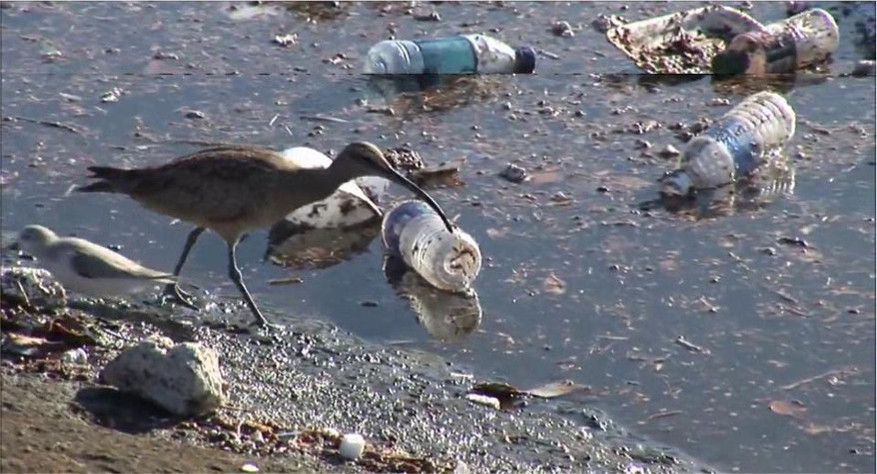
\includegraphics[keepaspectratio=true,width=\iwith]{images/matrix/701_11.jpg}}}&
%
\colorbox{white!0}{ \colorbox{red!70}{
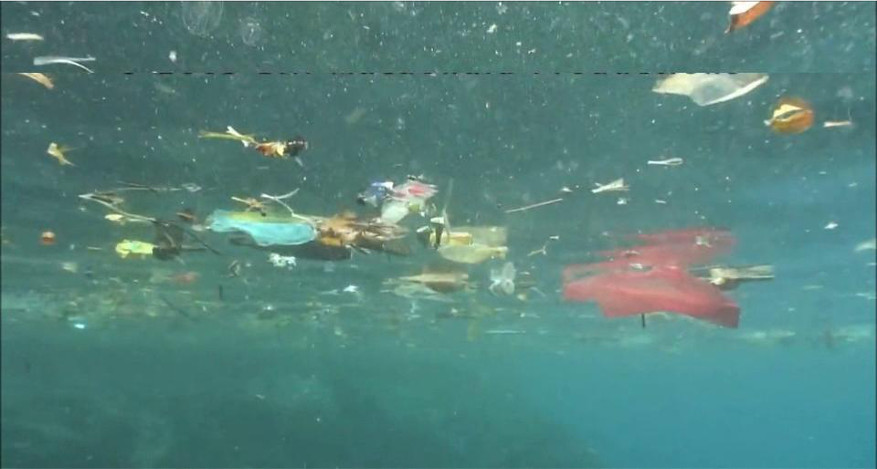
\includegraphics[keepaspectratio=true,width=\iwith]{images/matrix/6_01.jpg}}}
\end{tabular}}
\fi
\caption{Several images from the dataset: Left images are from the above water viewpoint and right images are from below water. A red border indicates an image classified as showing plastic, where a green border indicates an image classified as showing animals.}
\label{fig:datasetimages}
\end{figure}
\ifx\showpbreak\undefined \clearpage \fi
%\clearpage

\section{Method}
\label{sec:Method}
%This section describes the steps taken in this project. First the collection and the annotation of the dataset is explained. Thereafter the used algorithms are described in detail. The code used in this project can be found in appendix \ref{sec:ap-code}
This section describes the steps taken in this project.
First the pipeline is explained, after which the details of the implementation are stated.

\subsection{Pipeline}
\label{sec:Method-pipeline}
As stated in section \ref{sec:Theory} a Convolutional Neural Network has been used as a feature-vector of the image, after which a Support Vector Machine was used for classification.

Several libraries exist that implement a CNN.
In this project the choice is made to use Caffe \citep{jia2014caffe}.
This framework is open source and free to use.
Moreover it has a large community maintaining and developing, can run both on CPU and GPU and has an interface to \texttt{Python}.

The Caffe framework has several pre-trained CNNs.
In this project the Caffenet network is used, which is an implementation of Alexnet \citep{krizhevsky2012imagenet}. Caffenet is trained on the \textit{ilsvrc12} dataset, however in contrary to Alexnet, the order of pooling and normalisation is swapped. \citeneed

The output of Caffenet is a $1\times1000$ normalised vector, representing the confidence of the respective class.
However, the second-to-last layer of the network is used as feature-vector. This layer is a $10\times4096$ vector; $10$ rows because the network uses five overlapping `sub-images' (four corners and one centre) and their mirrored image, to improve accuracy.
Each row of $4096$ numbers is an abstract representation of the image, trained by the network.
To reduce complexity, the mean over the `sub-images' is used to compress the second-to-last layer data in a $1\times4096$ vector.

This 4096 dimensional vector is then used as the space for the SVM.
The three possible hyperplanes as described in section \ref{sec:Theory-class} were tested with several parameters.
Tests were conducted by training the SVM on the test-data, and using the validate-data to find the best parameters.

Three different types of hyperplanes were used.
A polygonal plane was tested with degrees of $2$ till $9$.
An RBF plane was tested with gammas of $0.0$ till $1.0$ with steps of $0.1$.
Lastly a linear plane was tested.
Each of the twenty SVM models were trained on part of the train-set, with intervals of order of magnitude; the sizes of the train-set were: 14, 140, 1400 and 14000 images.

\subsection{Impelemtation}
\label{sec:Method-implementation}
\Python has been used to write the code necessary for the pipeline.
Not only because Caffe has an interface in \Python, but also because of the many libraries available in \Python.

The library that allows the use of matrices and basic linear algebra operations is \texttt{numpy}.
Another library called \texttt{scikit.learn} has an implementation of an SVM, which has been used in this project.
The code used in this project can be found in appendix \ref{sec:ap-code}

All models are trained and tested on a laptop with 2$^{nd}$ generation i5 CPU, 4GB RAM and without using a GPU. Therefore time testing and training took in this project should be evaluated relatively to each other.

Furthermore, because no GPU was used, running Caffenet took a considerable amount of time. Therefore the output of the network had been saved for each image, to speed up the training of the SVM.

\subsection{Detecting location of plastic}
\label{sec:Method-location}
After testing the pipeline to detect plastic and marine life on images, small adaptations were made to find the location of the classes in the image.
When the system developed in this project is used for practical applications, location of the plastic is important.

To distinguish blobs in an image, several techniques could be used; however, as a prove of feasibility, no complex algorithms were used in this project.
A new piece of code was written that segments the image in sections and treats each of them as an image in the original pipeline.

The outcome of each segmented piece of the image are cumulated to show the confidence of detection of the classes at the given location in the image.

Because there is not labelled data of these segmented images, the evaluation could not be done on a large scale.
Therefore no sizeable experiments could be conducted to test the accuracy of locating of the classes.
However, in section \ref{sec:Results-location} the outcome of several tests is shown.











\iffalse
\subsection{Algorithm}
\label{sec:Method-algotihm}
\todo{structuur: -ding, -implementatie}
Because of the high accuracy Convolutional Neural Networks (CNNs) have reached on several problems in Computer Vision, they are also used in this project.
As stated in section \ref{sec:Method-Data}, this project will not train a CNN, but make use of a pre-trained one.
This not only because of the high chance of over-fitting on the data, but also because a pre-trained CNN has already learned basic visual concepts.
The first layers of a CNN consist of abstract representations of lines, corners and other gradients \citep{zeiler2014visualizing}.
Unnecessarily training a network on these concepts would be a waste of time.

Moreover floating plastic and animals, the classes that are trained in this project, consist of several distinctive features that are probably learnt by the network in higher layers of abstraction.
The second-to-last layer of the network consist of an abstract representation of the image.
This layer will probably have the information needed to classify the images. \citeneed

The output of this second-to-last layer will then be used to train several algorithms to research which will perform best.
The different algorithms are stated in detail below and the results of each algorithm can be found in tion}
After testing the pipeline to detect plastic and marine life on images, small adaptations were made tosection \ref{sec:Results} \todo{deze alinea uitbreiden}
\todo{pipeline en evaluatie }

\subsubsection{Convolutional Neural Network}
\label{sec:Method-CNN}
\todo{dit een stuk korter/vlotter/to-the-point (motivatie in theory)}
%How the algorithm from section CNN is used here... caffe framework (and why)...
In section \ref{sec:Theory-CNN} and \ref{sec:Method-Algorithm} the usage of Convolutional Neural Networks (CNNs) is funded.
In this section the chosen framework and network will be explained in detail.

Several libraries exist that implement a CNN.
In this project the choice is made to use Caffe \citep{jia2014caffe}.
This framework is open source and free to use.
Moreover it has a large community maintaining and developing, can run both on CPU and GPU and has an interface to \texttt{Python}.

The Caffe framework has several pre-trained CNNs.%, including GoogleNet.
However, to reduce computation needed, a smaller network called Caffenet.
This is an implementation of Alexnet \citet{krizhevsky2012imagenet} with small diferences, trained on the \textit{ilsvrc12} dataset. \citeneed
This network segments the image in five overlapping `sub-images' (four corners and one centre) and their mirrored image, to improve accuracy.

Every image in the dataset has been pulled through the network, after which the data of the last and second-to-last layer has been saved.
The data of the last layer of the network is returned as a \texttt{numpy}\footnote{\texttt{numpy} is a \texttt{Python} library used for linear algebra} array of size $1\times1000$.
The numbers in this array represent the probability the given image belongs to the respective class.
The second-to-last layer, called \textit{fc7} in this network, is a \texttt{numpy} array of size $10\times4096$.
The $4096$ columns are the abstract representation of the image, where the $10$ rows represent the different `sub-images'.
The data was stored on a hard-drive to speed-up further calculations.

%\subsubsection{Principal Component Analysis}
%\label{sec:Method-PCA}
%\todo{rede verzinnen waarom dit gedaan is}

\subsubsection{Feed Forward Network}
\label{sec:Method-FFN}
\todo{dit stuk weg}
To classify the second-to-last layer in the two classes of this project, a Feed Forward Neural Network (FFN) has been used.
This network has a structure of three layers: the input layer, the hidden layer and the output layer.
The implementation of this network has not been made in this project, but a \texttt{Python} implementation of \citeneed is used.
The input layer of 4096 nodes, one for each output of the CNN, and output layer of two nodes, one for each of the classes, were immutable.
Different numbers of nodes in the hidden layer were tested, even so the normalisation of the data.

The train-set has been used for training, and the validate-set has been used to distinguish between the different parameters.

The output of this network, shown in section \ref{sec:Results-FFN}, was not satisfactory, therefore the use of SVMs was researched further.

\subsubsection{Support Vector Machine}
\label{sec:Method-SVM}
After testing the FFN, the choice was made to use a Support Vector Machine (SVM).
In this case the implementation of \texttt{scikit.learn} of SVMs is used.
The second-to-last layer output constructs a 4096 dimensional space were the data represents points.
To speed up computation the mean of the `sub-images' is used to reduce the number of data-points.

The same method as with FFN regarding fitting the data and parameters on the train- and validate-set was used.
The results are shown in section \ref{sec:Results-SVM}.

\subsubsection{Detecting location of plastic}
\label{sec:Method-sub}
After several tests with a SVM, locating plastic within the image was researched.
Several techniques could be used to distinguish blobs, however, as a prove of feasibility, no complex algorithms were used.
A new piece of code was written that segments the image in sections and treats each of them as an image in the original pipeline.

Because there is not labelled data of these segmented images, the evaluation could not be done on a large scale.
Therefore no sizable experiments could be conducted to test the accuracy of locating of the classes.
However, in section \ref{sec:Results-sub} the outcome of several test is shown.

\fi
\ifx\showpbreak\undefined \newpage \fi

\section{Results}
\label{sec:Results}
In this section the outcome of the tests is shown.
Both the search for optimal parameters of the SVM and the outcome of several tests using the localisation of plastic are described below.
%In this section part of the output of the \texttt{Python} code is located.
%The full tables of output can be found in Appendix \ref{sec:ap-out}, however, only the more interesting parts are shown in this section.


%\subsection{Principal Component Analysis}
%\label{sec:Results-PCA}
%...amount of principal components of 1000...

%\subsection{Feed Forward Network}
%\label{sec:Results-FFN}
%Several different parameters of the Feed Forward Network were used.
%However, the output of each run is always the same, irrespectively the input-vector.

\subsection{Pipeline}
\label{sec:Results-SVM}
The outcome of the different parameters the pipeline was tested with can be found in appendix \ref{sec:ap-out}.
Several details of the raw output are visualised and shown in this section.
The accuracy shown in this section is calculated by dividing the correct labelled images by the total amount of images. The formula below shows this calculation:
\[
\frac{\#(Outcome_{True}\,and\,Label_{True})+\#(Outcome_{False}\,and\,Label_{False})}{\#tested\,images}
\]

The time the training and testing of the SVM took was calculated by using the difference in \textit{System time} from start to finish of a run.
Because the data from the CNN was saved on a hard drive and imported in RAM, that time is not included in these tests.

Figure \ref{fig:c14} shows how each of the SVM models perform and what time it took to train and test.
All these tests were fitted on the data of the under-water viewpoint.
The blue dots represent the accuracy, which can be read out on the left y-axis.
The green and red bars represent time taken to train and test respectively, that can be read out on the right y-axis.
Each instance on the x-axis is one of the twenty different hyperplanes.
The graphs show how the accuracy increases with larger train-sets. However, the RBF kernel -- irrespectively to $\gamma$ -- never reaches a satisfactory accuracy, while needing much time to train. On the other hand, the linear kernel shows a high accuracy while using a small amount of time to train and test. The polynomial kernel shows a decrease in accuracy with higher degrees.

In figure \ref{fig:lin1} the results of the orders of magnitude of the train size are shown when a linear SVM was used. The figure consists of two graphs, the left one showing the accuracy on each class individually and the total accuracy, the right one showing the time taken to test and train. The x-axis shows the size of the train-set on a logarithmic scale.
In other words, the first column of the first four graphs is plotted in a single image, only using a different set of test-data.
This figure shows how the accuracy of the individual classes is higher than the combination. It shows an increase in accuracy with larger train-sets while also increasing the time needed to train.

\ifx\showmixi\undefined
In figure \ref{fig:lin3} a test that accounts for possible overfitting was executed. These tests were trained on one train-set of one of both viewpoints, and tested on the test-set of the other viewpoint. These graphs show a low accuracy for recognising the animal class and therefore a low accuracy on both. The plastic class however does shows a better accuracy between the 70\% and 90\%.
\fi

Figure \ref{fig:lin2} shows a graph of the final model, this is also a linear SVM tested on several orders of magnitude of train data.
The tests in this figure were conducted on a combination of both viewpoints.
These results show the same trend as the graphs in figure \ref{fig:lin1}.

\begin{figure}%[h!tb]
\centering
\ifx\showfig\undefined
\centerline{
\begin{tikzpicture}
%\begin{semilogyaxis}[
\begin{axis}[
    title={Time and accuracy of different SVM settings with n=14, n=140, n=1400 and n-14000},
    width=\widefigwidth,
    height=\mgraphheight,
    ymin=0, ymax=2,
    %xmin=0,xmax=21,
	xtick={0,...,21},
	xticklabels={
		%linear,poly:d=2,poly:d=3,poly:d=4,poly:d=5,poly:d=6,poly:d=7,poly:d=8,poly:d=9,rbf:$\gamma$=0.0,rbf:$\gamma$=0.1,rbf:$\gamma$=0.2,rbf:$\gamma$=0.3,rbf:$\gamma$=0.4,rbf:$\gamma$=0.5,rbf:$\gamma$=0.6,rbf:$\gamma$=0.7,rbf:$\gamma$=0.8,rbf:$\gamma$=0.9,rbf:$\gamma$=1.0,
        linear,$\,$,d=2,d=3,d=4,d=5,d=6,d=7,d=8,d=9,$\,$,
        $\gamma$=0.0,$\gamma$=0.1,$\gamma$=0.2,$\gamma$=0.3,$\gamma$=0.4,$\gamma$=0.5,$\gamma$=0.6,
        $\gamma$=0.7,$\gamma$=0.8,$\gamma$=0.9,$\gamma$=1.0,
	},
	x tick label style={rotate=30, anchor=north east, inner sep=0mm},
	xlabel={\hspace{1cm}${\underbrace{\text{\hspace{5cm}}}\atop\text{polynomial}}$\hspace{0.4cm}${\underbrace{\text{\hspace{7cm}}}\atop\text{rbf}}$},
	xlabel style={at={(0.5,-0.03)}},
	ylabel=Time (sec),
	axis y line*=right,
	enlargelimits=0.05,
	legend style={at={(0.5,-0.4)},
	anchor=north,legend columns=-1},
	ybar stacked,
	ylabel near ticks
]
\addplot[color=orange!80,fill=orange!80]
	coordinates {
	(0,0.0) (2,0.0) (3,0.0) (4,0.0) (5,0.0) (6,0.0) (7,0.0) (8,0.0) (9,0.0) (11,0.0) (12,0.0) (13,0.0) (14,0.0) (15,0.0) (16,0.0) (17,0.0) (18,0.0) (19,0.0) (20,0.0) (21,0.0) 
    };
\addplot[color=purple!60,fill=purple!70]
    coordinates {
    (0,0.6) (2,0.7) (3,1.0) (4,1.0) (5,0.8) (6,1.2) (7,0.9) (8,1.2) (9,1.1) (11,0.9) (12,0.8) (13,1.2) (14,1.2) (15,1.0) (16,1.2) (17,0.8) (18,0.8) (19,1.2) (20,0.7) (21,0.7)
    };
%\end{semilogyaxis}
\end{axis}
\begin{axis}[
    width=\widefigwidth,
    height=\mgraphheight,
    ymin=0,ymax=1,
   % xmin=0,xmax=21,
    x tick label style={color=white},
	ylabel={Accuracy ($\frac{correct}{total}$)},
	axis y line*=left,
	enlargelimits=0.05,
	legend style={at={(0.5,-0.4)},
	anchor=north,legend columns=-1},
	ylabel near ticks,
	ymajorgrids=true,
	xmajorgrids=false,
    grid style=dashed
]
%\addlegendimage{blue, mark=*}
%\addlegendimage{only marks, orange!80, mark=square*}
%\addlegendimage{only marks, purple!70, mark=square*}
%\legend{Accuracy, Train time, Test time}
\addplot[mark=*,blue,jump mark mid]
	coordinates {
	(-1,-10) (0,0.571) (1,-10) (2,0.555) (3,0.533) (4,0.432) (5,0.378) (6,0.479) (7,0.600) (8,0.590) (9,0.589) (10,-10) (11,0.570) (12,0.570) (13,0.570) (14,0.190) (15,0.172) (16,0.164) (17,0.160) (18,0.158) (19,0.154) (20,0.153) (21,0.153) (22,-10)
    };
\end{axis}
\end{tikzpicture}
}
\vspace{-.2cm}
\centerline{
\begin{tikzpicture}
%\begin{semilogyaxis}[
\begin{axis}[
    %title={Time and accuracy of different SVM settings with n=140},
    width=\widefigwidth,
    height=\mgraphheight,
    ymin=0, ymax=20,
    %xmin=0,xmax=21,
	x tick label style={color=white},
	xlabel style={at={(0.5,-0.03)}},
	ylabel=Time (sec),
	axis y line*=right,
	enlargelimits=0.05,
	legend style={at={(0.5,-0.4)},
	anchor=north,legend columns=-1},
	ybar stacked,
	ylabel near ticks
]
\addplot[color=orange!80,fill=orange!80]
	coordinates {
	(0,0.2) (2,0.4) (3,0.5) (4,0.4) (5,0.4) (6,0.6) (7,0.6) (8,0.4) (9,0.6) (11,0.4) (12,0.4) (13,0.6) (14,0.6) (15,0.6) (16,0.6) (17,0.4) (18,0.4) (19,0.6) (20,0.4) (21,0.4) 
    };
\addplot[color=purple!70,fill=purple!70]
    coordinates {
    (0,3.1) (2,4.5) (3,5.6) (4,6.3) (5,7.1) (6,7.5) (7,7.7) (8,7.6) (9,8.3) (11,7.2) (12,7.2) (13,10.3) (14,10.1) (15,9.5) (16,10.4) (17,7.8) (18,7.1) (19,10.4) (20,6.4) (21,6.8) 
    };
%\end{semilogyaxis}
\end{axis}
\begin{axis}[
    width=\widefigwidth,
    height=\mgraphheight,
    ymin=0,ymax=1,
   % xmin=0,xmax=21,
    xtick={0,...,21},
	xticklabels={
		%linear,poly:d=2,poly:d=3,poly:d=4,poly:d=5,poly:d=6,poly:d=7,poly:d=8,poly:d=9,rbf:$\gamma$=0.0,rbf:$\gamma$=0.1,rbf:$\gamma$=0.2,rbf:$\gamma$=0.3,rbf:$\gamma$=0.4,rbf:$\gamma$=0.5,rbf:$\gamma$=0.6,rbf:$\gamma$=0.7,rbf:$\gamma$=0.8,rbf:$\gamma$=0.9,rbf:$\gamma$=1.0,
        linear,$\,$,2,3,4,5,6,7,8,9,$\,$,0.0,0.1,0.2,0.3,0.4,0.5,0.6,0.7,0.8,0.9,1.0,
	},
	x tick label style={font=\scriptsize},%rotate=30, anchor=north east, inner sep=0mm},
	xlabel={\hspace{1cm}${\underbrace{\text{\hspace{3.5cm}}}\atop\text{polynomial (d)}}$\hspace{0.6cm}${\underbrace{\text{\hspace{5cm}}}\atop\text{rbf (}\gamma\text{)}}$},
	xlabel style={at={(0.5,0.1)}},
	ylabel={Accuracy ($\frac{correct}{total}$)},
	axis y line*=left,
	enlargelimits=0.05,
	legend style={at={(0.5,-0.4)},
	anchor=north,legend columns=-1},
	ylabel near ticks,
	ymajorgrids=true,
	xmajorgrids=false,
    grid style=dashed
]
%\addlegendimage{blue, mark=*}
%\addlegendimage{only marks, orange!80, mark=square*}
%\addlegendimage{only marks, purple!70, mark=square*}
%\legend{Accuracy, Train time, Test time}
\addplot[mark=*,blue,jump mark mid]
	coordinates {
	(-1,-10) (0,0.898) (1,-10) (2,0.917) (3,0.910) (4,0.896) (5,0.883) (6,0.868) (7,60.853) (8,0.841) (9,0.831) (10,-10) (11,0.599) (12,0.553) (13,0.553) (14,0.553) (15,0.553) (16,0.553) (17,0.553) (18,0.553) (19,0.553) (20,0.553) (21,0.553) (22,-10)
    };
\end{axis}
\node [black] (trainsize) at (1.0,3.0) {\it train-size=140};
\end{tikzpicture}
}
\vspace{-.2cm}
\centerline{
\begin{tikzpicture}
%\begin{semilogyaxis}[
\begin{axis}[
    %title={Time and accuracy of different SVM settings with n=1400},
    width=1.3\textwidth,
    height=.22\textheight,
    ymin=0, ymax=200,
    %xmin=0,xmax=21,
	xtick={0,...,21},
	xticklabels={
		%linear,poly:d=2,poly:d=3,poly:d=4,poly:d=5,poly:d=6,poly:d=7,poly:d=8,poly:d=9,rbf:$\gamma$=0.0,rbf:$\gamma$=0.1,rbf:$\gamma$=0.2,rbf:$\gamma$=0.3,rbf:$\gamma$=0.4,rbf:$\gamma$=0.5,rbf:$\gamma$=0.6,rbf:$\gamma$=0.7,rbf:$\gamma$=0.8,rbf:$\gamma$=0.9,rbf:$\gamma$=1.0,
        linear,$\,$,d=2,d=3,d=4,d=5,d=6,d=7,d=8,d=9,$\,$,
        $\gamma$=0.0,$\gamma$=0.1,$\gamma$=0.2,$\gamma$=0.3,$\gamma$=0.4,$\gamma$=0.5,$\gamma$=0.6,
        $\gamma$=0.7,$\gamma$=0.8,$\gamma$=0.9,$\gamma$=1.0,
	},
	x tick label style={rotate=30, anchor=north east, inner sep=0mm},
	xlabel={\hspace{1cm}${\underbrace{\text{\hspace{5cm}}}\atop\text{polynomial}}$\hspace{0.4cm}${\underbrace{\text{\hspace{7cm}}}\atop\text{rbf}}$},
	xlabel style={at={(0.5,-0.03)}},
	ylabel=Time (sec),
	axis y line*=right,
	enlargelimits=0.05,
	legend style={at={(0.5,-0.4)},
	anchor=north,legend columns=-1},
	ybar stacked,
	ylabel near ticks
]
\addplot[color=orange!80,fill=orange!80]
	coordinates {
	(0,5.6) (2,10.1) (3,14.1) (4,13.0) (5,12.7) (6,20.6) (7,22.8) (8,16.1) (9,23.2) (11,29.8) (12,64.7) (13,58.7) (14,57.6) (15,58.6) (16,58.2) (17,51.7) (18,50.9) (19,48.9) (20,54.5) (21,54.2) 
    };
\addplot[color=purple!70,fill=purple!70]
    coordinates {
    (0,8.3) (2,17.2) (3,20.5) (4,17.1) (5,18.8) (6,30.3) (7,32.9) (8,23.3) (9,38.5) (11,40.6) (12,93.2) (13,77.5) (14,79.9) (15,82.3) (16,82.1) (17,91.9) (18,83.2) (19,87.9) (20,45.1) (21,78.5) 
    };
%\end{semilogyaxis}
\end{axis}
\begin{axis}[
    width=1.3\textwidth,
    height=.22\textheight,
    ymin=0,ymax=1,
   % xmin=0,xmax=21,
    x tick label style={color=white},
	ylabel={Accuracy ($\frac{correct}{total}$)},
	axis y line*=left,
	enlargelimits=0.05,
	legend style={at={(0.5,-0.4)},
	anchor=north,legend columns=-1},
	ylabel near ticks,
	ymajorgrids=true,
	xmajorgrids=false,
    grid style=dashed
]
%\addlegendimage{blue, mark=*}
%\addlegendimage{only marks, orange!80, mark=square*}
%\addlegendimage{only marks, purple!70, mark=square*}
%\legend{Accuracy, Train time, Test time}
\addplot[mark=*,blue,jump mark mid]
	coordinates {
	(-1,-10) (0,0.993) (1,-10) (2,0.994) (3,0.994) (4,0.993) (5,0.992) (6,0.991) (7,0.986) (8,0.982) (9,0.977) (10,-10) (11,0.990) (12,0.553) (13,0.553) (14,0.553) (15,0.553) (16,0.553) (17,0.553) (18,0.553) (19,0.553) (20,0.553) (21,0.553) (22,-10)
    };
\end{axis}
\end{tikzpicture}
}
\vspace{-.2cm}
\centerline{
\begin{tikzpicture}
%\begin{semilogyaxis}[
\begin{axis}[
    %title={Time and accuracy of different SVM settings with n=14000},
    width=\widefigwidth,
    height=\mgraphheight,
    ymin=0, ymax=30000,
    %xmin=0,xmax=21,
	xtick={0,...,21},
	xticklabels={
		%linear,poly:d=2,poly:d=3,poly:d=4,poly:d=5,poly:d=6,poly:d=7,poly:d=8,poly:d=9,rbf:$\gamma$=0.0,rbf:$\gamma$=0.1,rbf:$\gamma$=0.2,rbf:$\gamma$=0.3,rbf:$\gamma$=0.4,rbf:$\gamma$=0.5,rbf:$\gamma$=0.6,rbf:$\gamma$=0.7,rbf:$\gamma$=0.8,rbf:$\gamma$=0.9,rbf:$\gamma$=1.0,
        linear,$\,$,d=2,d=3,d=4,d=5,d=6,d=7,d=8,d=9,$\,$,
        $\gamma$=0.0,$\gamma$=0.1,$\gamma$=0.2,$\gamma$=0.3,$\gamma$=0.4,$\gamma$=0.5,$\gamma$=0.6,
        $\gamma$=0.7,$\gamma$=0.8,$\gamma$=0.9,$\gamma$=1.0,
	},
	x tick label style={rotate=30, anchor=north east, inner sep=0mm},
	xlabel={\hspace{1cm}${\underbrace{\text{\hspace{5cm}}}\atop\text{polynomial}}$\hspace{0.4cm}${\underbrace{\text{\hspace{7cm}}}\atop\text{rbf}}$},
	xlabel style={at={(0.5,-0.03)}},
	ylabel=Time (sec),
	axis y line*=right,
	enlargelimits=0.05,
	%legend style={at={(0.5,2.2)},anchor=north,legend columns=-1},
	ybar stacked,
	ylabel near ticks,
	scale ticks above exponent={5}
]
\addplot[color=orange!80,fill=orange!80]
	coordinates {
	(0,74.6) (2,1124.4) (3,2068.0) (4,3331.6) (5,4678.5) (6,5198.9) (7,5282.2) (8,5193.3) (9,5083.9) (11,586.3) (12,24560.3) (13,25139.6) (14,25104.7) (15,25389.9) (16,24877.4) (17,26216.1) (18,25266.2) (19,26166.7) (20,18654.6) (21,16250.9)
    };
\addplot[color=purple!70,fill=purple!70]
    coordinates {
    (0,8.4) (2,155.7) (3,277.0) (4,459.8) (5,646.8) (6,696.6) (7,706.6) (8,719.4) (9,714.2) (11,86.2) (12,1067.4) (13,1069.5) (14,1059.1) (15,1052.6) (16,1055.4) (17,1062.9) (18,618.3) (19,1072.2) (20,607.0) (21,399.1)
    };
%\end{semilogyaxis}
\end{axis}
\begin{axis}[
    width=\widefigwidth,
    height=\mgraphheight,
    ymin=0,ymax=1,
   % xmin=0,xmax=21,
    x tick label style={color=white},
	ylabel={Accuracy ($\frac{correct}{total}$)},
	axis y line*=left,
	enlargelimits=0.05,
	legend style={at={(0.5,-0.5)},
	anchor=north,legend columns=-1},
	ylabel near ticks,
	ymajorgrids=true,
	xmajorgrids=false,
    grid style=dashed,
]
\addlegendimage{blue, mark=*}
\addlegendimage{only marks, orange!80, mark=square*}
\addlegendimage{only marks, purple!70, mark=square*}
\legend{Accuracy, Train time, Val time}
\addplot[mark=*,blue,jump mark mid]
	coordinates {
	(-1,-10) (0,0.999) (1,-10) (2,0.978) (3,0.964) (4,0.862) (5,0.741) (6,0.606) (7,0.578)
    (8,0.569) (9,0.561) (10,-10) (11,0.991) (12,0.597) (13,0.559) (14,0.554)
    (15,0.554) (16,0.554) (17,0.554) (18,0.554) (19,0.554) (20,0.554)
    (21,0.553) (22,-10)
    };
\end{axis}
\end{tikzpicture}
} \fi
\caption{Outcome of the different parameters of the SVM trained on different slices of train-data and tested on the validation-set. The linear kernel has one of the highest accuracies, while using the least time to train. Opposing to the trend of the RBF kernel}
\label{fig:c14}
\end{figure}


\begin{figure}%[h!tb]
\centering
\ifx\showfig\undefined
\centerline{
\begin{minipage}{1.3\textwidth}
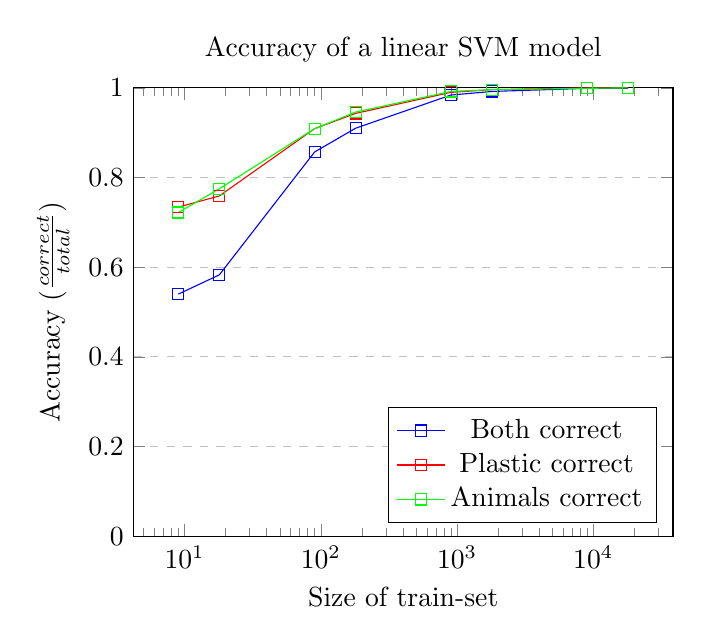
\begin{tikzpicture}
\begin{semilogxaxis}[
    title={Accuracy of a linear SVM model},
    xlabel={Size of train-set},
    ylabel={Accuracy ($\frac{correct}{total}$)},
    %xmin=0, xmax=18000,
    ymin=0, ymax=1,
    legend pos=south east,
    ymajorgrids=true,
    grid style=dashed,
]
\addplot[
    color=blue,
    mark=square,
    ]
    coordinates {
    %(14,0.571)(140,0.898)(1400,0.993)(14000,0.999)
     (9,0.540) (18,0.583) (90,0.857) (180,0.910) (900,0.984) (1800,0.992) (9000,0.999) (18000,0.999)
    };
    \addlegendentry{Both correct}
\addplot[
    color=red,
    mark=square,
    ]
    coordinates {
    (9,0.734) (18,0.759) (90,0.909) (180,0.943) (900,0.990) (1800,0.996) (9000,1.000) (18000,1.000)
    %(14,0.741)(140,0.947)(1400,0.996)(14000,1.000)
    };
    \addlegendentry{Plastic correct}
\addplot[
    color=green,
    mark=square,
    ]
    coordinates {
    (9,0.722) (18,0.775) (90,0.909) (180,0.946) (900,0.992) (1800,0.996) (9000,0.999) (18000,1.000)
    %(14,0.766)(140,0.924)(1400,0.997)(14000,0.999)
    };
    \addlegendentry{Animals correct}
\end{semilogxaxis}
\end{tikzpicture}
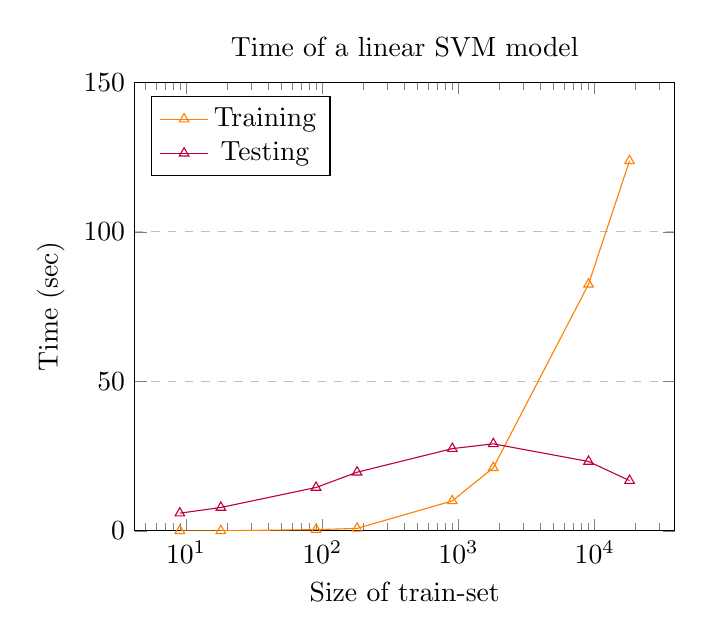
\begin{tikzpicture}
\begin{semilogxaxis}[
    title={Time of a linear SVM model},
    xlabel={Size of train-set},
    ylabel={Time (sec)},
    %xmin=0, xmax=18000,
    ymin=0, ymax=150,
    legend pos=north west,
    ymajorgrids=true,
    grid style=dashed,
    ]
\addplot[
    color=orange,
    mark=triangle,
    ]
    coordinates {
    (9,0.0) (18,0.0) (90,0.4) (180,0.8) (900,10.0) (1800,21.1) (9000,82.5) (18000,123.8)
    %(14,0.0)(140,0.2)(1400,5.6)(14000,74.6)
    };
    \addlegendentry{Training}
\addplot[
    color=purple,
    mark=triangle,
    ]
    coordinates {
    (9,5.9) (18,7.8) (90,14.5) (180,19.6) (900,27.5) (1800,29.1) (9000,23.2) (18000,16.8)
    %(14,0.6)(140,3.1)(1400,8.3)(14000,8.4)
    };
    \addlegendentry{Testing} 
\end{semilogxaxis}
\end{tikzpicture}
\end{minipage}
} \fi
\caption{Graph of time and accuracy of a linear SVM on different sizes of data from the under water viewpoint. The test-data consisted of 4.123 images. Large datasets show a high accuracy, however even small amounts of data show satisfying results.}
\label{fig:lin1}
\end{figure}

\ifx\showmixi\undefined
\begin{figure}%[h!tb]
\centering
\ifx\showfig\undefined
\resizebox{\textwidth}{!}{
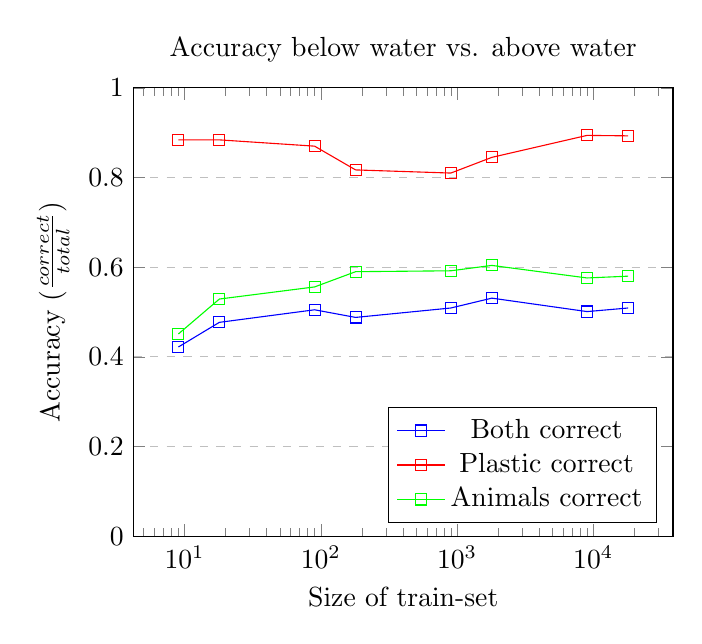
\begin{tikzpicture}
\begin{semilogxaxis}[
    title={Accuracy below water vs. above water},
    xlabel={Size of train-set},
    ylabel={Accuracy ($\frac{correct}{total}$)},
    %xmin=0, xmax=18000,
    ymin=0, ymax=1,
    legend pos=south east,
    ymajorgrids=true,
    grid style=dashed,
]
\addplot[
    color=blue,
    mark=square,
    ]
    coordinates {
    (9,0.422) (18,0.477) (90,0.505) (180,0.488) (900,0.509) (1800,0.531) (9000,0.501) (18000,0.509)
    };
    \addlegendentry{Both correct}
\addplot[
    color=red,
    mark=square,
    ]
    coordinates {
    (9,0.884) (18,0.884) (90,0.870) (180,0.817) (900,0.810) (1800,0.845) (9000,0.894) (18000,0.893)
    };
    \addlegendentry{Plastic correct}
\addplot[
    color=green,
    mark=square,
    ]
    coordinates {
    (9,0.451) (18,0.529) (90,0.556) (180,0.590) (900,0.592) (1800,0.604) (9000,0.576) (18000,0.580)
    };
    \addlegendentry{Animals correct}
\end{semilogxaxis}
\end{tikzpicture}
\hspace{.5cm}
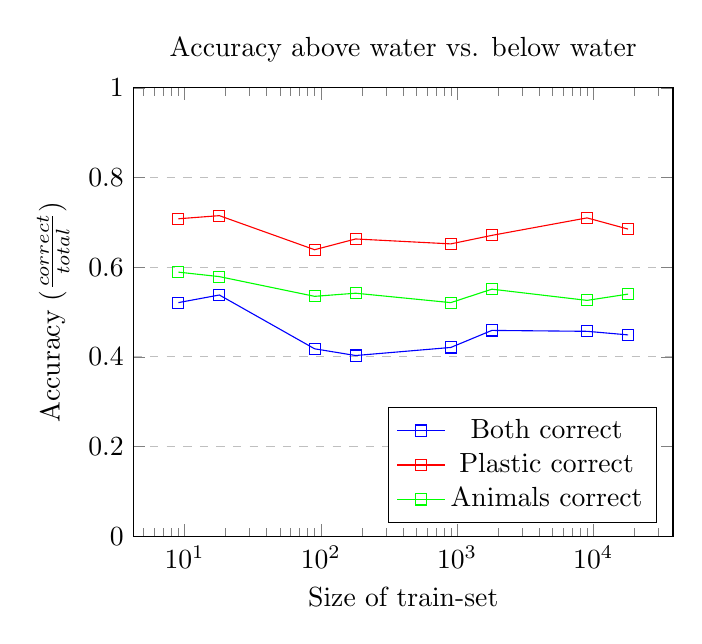
\begin{tikzpicture}
\begin{semilogxaxis}[
    title={Accuracy above water vs. below water},
    xlabel={Size of train-set},
    ylabel={Accuracy ($\frac{correct}{total}$)},
    %xmin=0, xmax=18000,
    ymin=0, ymax=1,
    legend pos=south east,
    ymajorgrids=true,
    grid style=dashed,
]
\addplot[
    color=blue,
    mark=square,
    ]
    coordinates {
    (9,0.521) (18,0.538) (90,0.418) (180,0.403) (900,0.421) (1800,0.459) (9000,0.457) (18000,0.449)
    };
    \addlegendentry{Both correct}
\addplot[
    color=red,
    mark=square,
    ]
    coordinates {
    (9,0.708) (18,0.715) (90,0.639) (180,0.663) (900,0.652) (1800,0.671) (9000,0.710) (18000,0.685)
    };
    \addlegendentry{Plastic correct}
\addplot[
    color=green,
    mark=square,
    ]
    coordinates {
    (9,0.589) (18,0.579) (90,0.535) (180,0.542) (900,0.521) (1800,0.551) (9000,0.526) (18000,0.540)
    };
    \addlegendentry{Animals correct}
\end{semilogxaxis}
\end{tikzpicture}
} \fi
\caption{Graph of time and accuracy of a linear SVM on different sizes of data. The test set and train set came from the different datasets. The animal class does not gain high accuracy, the plastic class does.}
\label{fig:lin3}
\end{figure}
\fi

\begin{figure}%[h!tb]
\centering
\ifx\showfig\undefined
\centerline{
\begin{minipage}{1.3\textwidth}
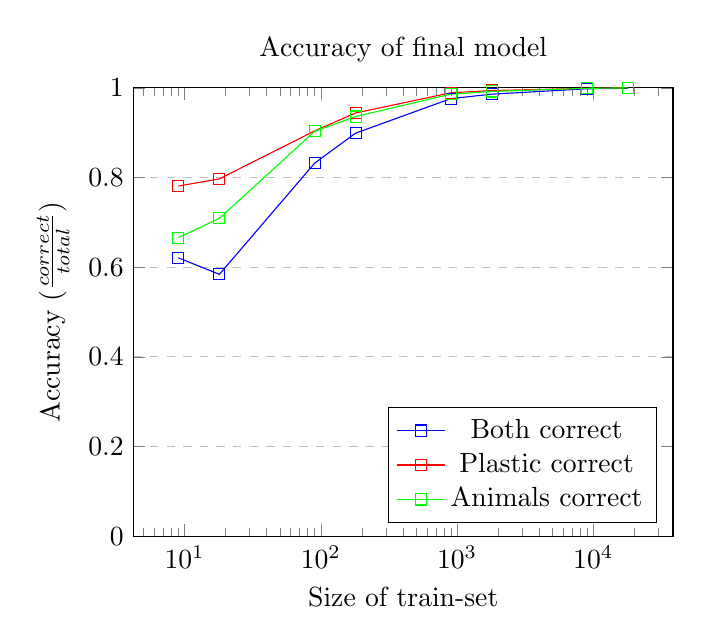
\begin{tikzpicture}
\begin{semilogxaxis}[
    title={Accuracy of final model},
    xlabel={Size of train-set},
    ylabel={Accuracy ($\frac{correct}{total}$)},
    %xmin=0, xmax=18000,
    ymin=0, ymax=1,
    legend pos=south east,
    ymajorgrids=true,
    grid style=dashed,
]
\addplot[
    color=blue,
    mark=square,
    ]
    coordinates {
    (9,0.621)(18,0.584)(90,0.832)(180,0.899)(900,0.976)(1800,0.986)(9000,0.998)(18000,0.999)
    };
    \addlegendentry{Both correct}
\addplot[
    color=red,
    mark=square,
    ]
    coordinates {
    (9,0.781)(18,0.797)(90,0.904)(180,0.944)(900,0.989)(1800,0.994)(9000,0.999)(18000,1.000)
    };
    \addlegendentry{Plastic correct}
\addplot[
    color=green,
    mark=square,
    ]
    coordinates {
    (9,0.666)(18,0.709)(90,0.903)(180,0.936)(900,0.986)(1800,0.992)(9000,0.999)(18000,1.000)
    };
    \addlegendentry{Animals correct}
\end{semilogxaxis}
\end{tikzpicture}
\hspace{.5cm}
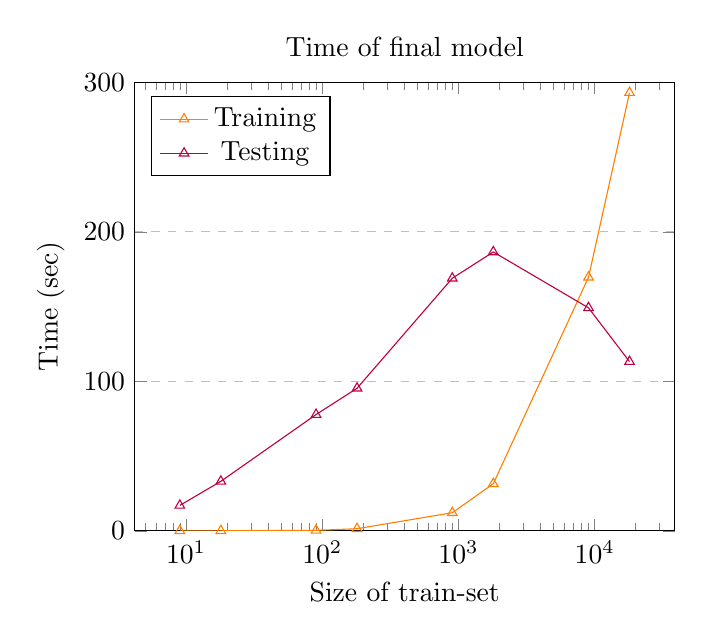
\begin{tikzpicture}
\begin{semilogxaxis}[
    title={Time of final model},
    xlabel={Size of train-set},
    ylabel={Time (sec)},
    %xmin=0, xmax=18000,
    ymin=0, ymax=300,
    legend pos=north west,
    ymajorgrids=true,
    grid style=dashed,
    ]
\addplot[
    color=orange,
    mark=triangle,
    ]
    coordinates {
    (9,0.0)(18,0.0)(90,0.3)(180,1.4)(900,12.1)(1800,31.5)(9000,169.7)(18000,293.2)
    };
    \addlegendentry{Training}
\addplot[
    color=purple,
    mark=triangle,
    ]
    coordinates {
    (9,17.0)(18,33.1)(90,77.8)(180,95.4)(900,169.0)(1800,186.6)(9000,149.2)(18000,113.2)
    };
    \addlegendentry{Testing} 
\end{semilogxaxis}
\end{tikzpicture}
\end{minipage}
} \fi
\caption{Graph of time and accuracy of a linear SVM on different sizes of data from a set of mixed images of the above and below water viewpoint. The test-data consisted of 18.583 images. The same trend as the graphs in figure \ref{fig:lin1} is seen.}
\label{fig:lin2}
\end{figure}

\subsection{Detecting the location of plastic}
\label{sec:Results-location}
As stated in section \ref{sec:Method-location}, the localisation of plastic within the image could not be evaluated truly.
However, several images were pulled through the pipeline and the results can be seen in figure \ref{fig:sub-matrix}.
The middle column in the figure shows the tested images.
The more red is showing in the figure on the right, the more confidence the program has in detecting plastic on that location in the image.
The images on the left represent the same with the greenness for locating animals.
Testing the localisation took a considerable amount of time, because a run through the pipeline could take up to $5$ seconds per sub-image.
Because these tests were conducted on a pyramid-segmentation of depth 4, a total amount of 341 images were run through the pipeline per test.

The results show that the confidence of detecting plastic or animals within the image does not always agree with what is shown in the original image.
However, because of the lack of annotation, there is no manner in which these results can evaluated more thoroughly.

\begin{figure}%[h!tb]
\centering
\ifx\showfig\undefined
\def\segwidth{.22\textwidth}
\begin{tabular}{ccc}

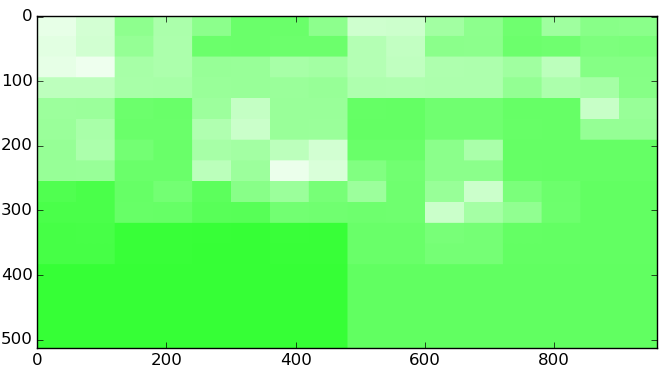
\includegraphics[keepaspectratio=true,width=\segwidth]{images/segment/6_01__animals__.png} &
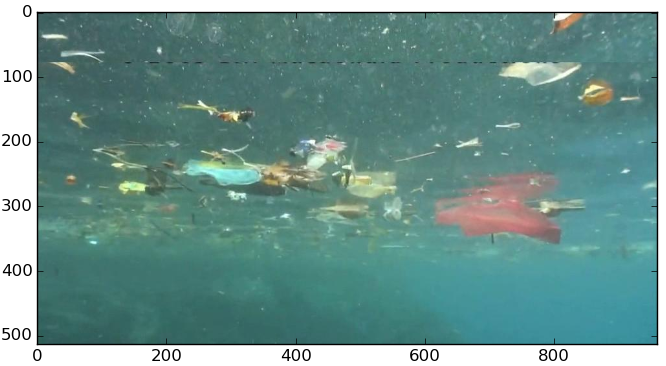
\includegraphics[keepaspectratio=true,width=\segwidth]{images/segment/6_01__image__.png} &
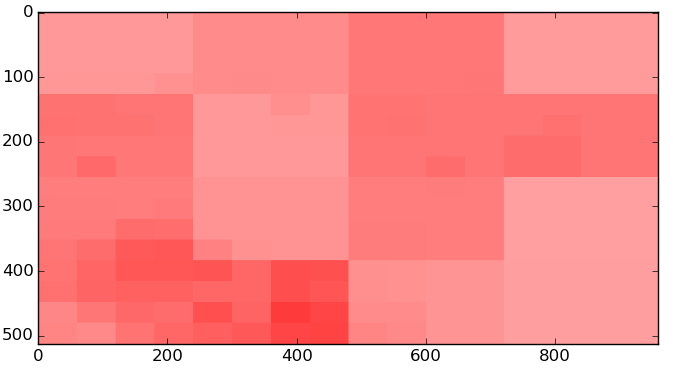
\includegraphics[keepaspectratio=true,width=\segwidth]{images/segment/6_01__plastic__.png} \\

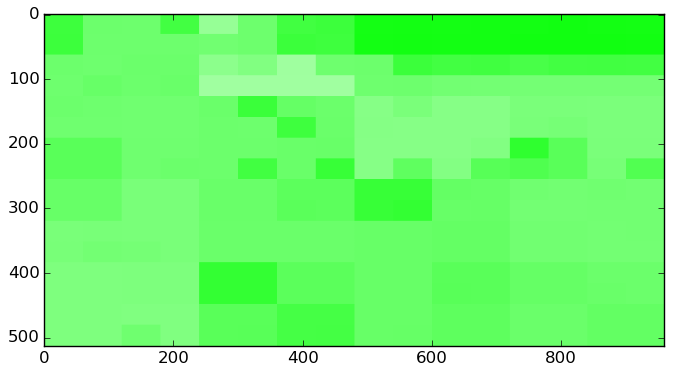
\includegraphics[keepaspectratio=true,width=\segwidth]{images/segment/31_11__animals__.png} &
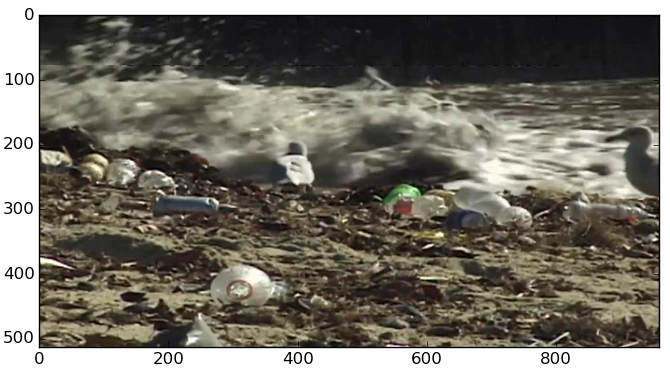
\includegraphics[keepaspectratio=true,width=\segwidth]{images/segment/31_11__image__.png} &
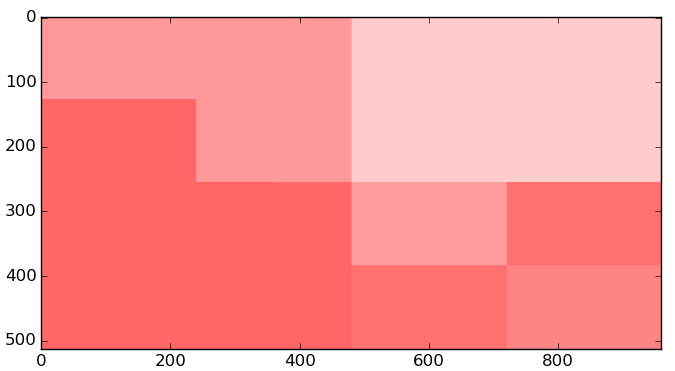
\includegraphics[keepaspectratio=true,width=\segwidth]{images/segment/31_11__plastic__.png} \\

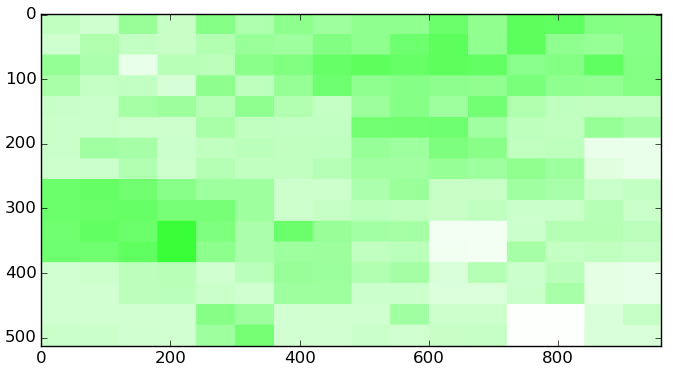
\includegraphics[keepaspectratio=true,width=\segwidth]{images/segment/253_01__animals__.png} &
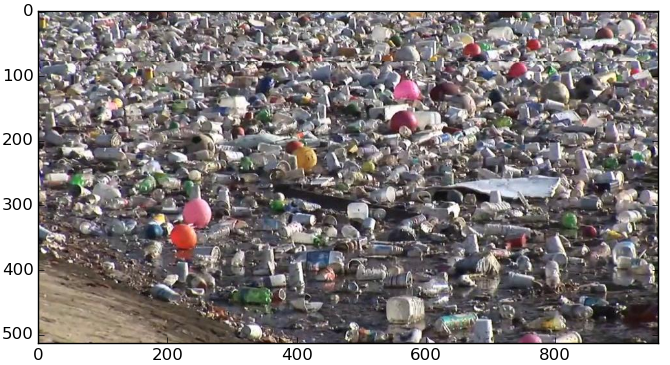
\includegraphics[keepaspectratio=true,width=\segwidth]{images/segment/253_01__image__.png} &
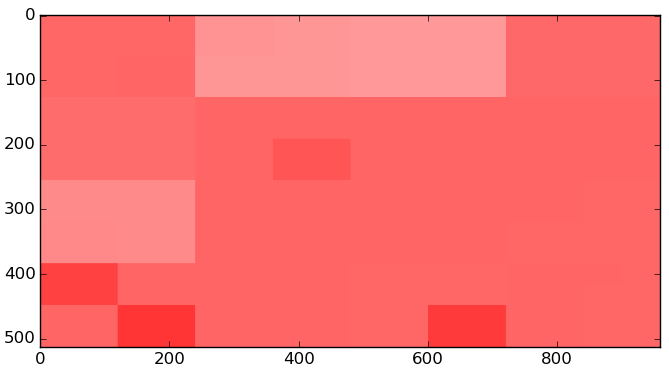
\includegraphics[keepaspectratio=true,width=\segwidth]{images/segment/253_01__plastic__.png} \\

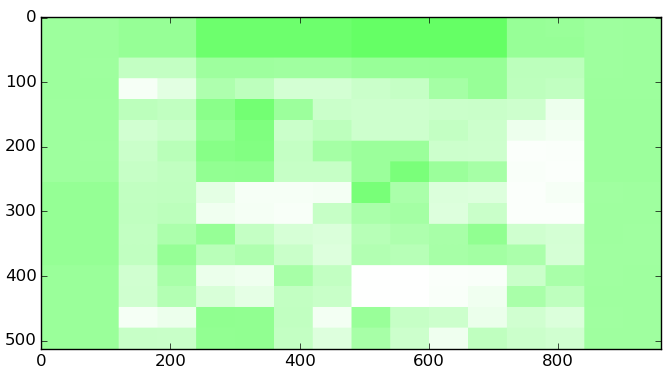
\includegraphics[keepaspectratio=true,width=\segwidth]{images/segment/299_00__animals__.png} &
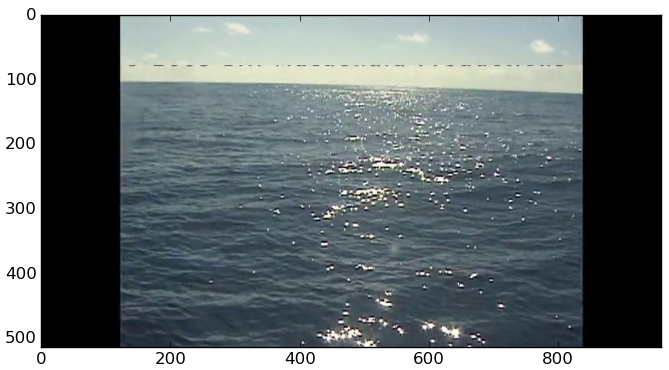
\includegraphics[keepaspectratio=true,width=\segwidth]{images/segment/299_00__image__.png} &
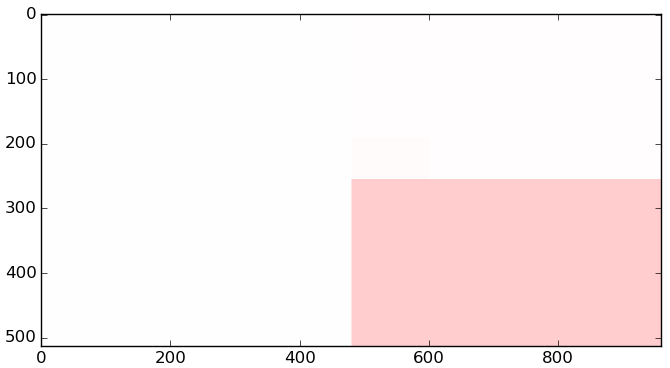
\includegraphics[keepaspectratio=true,width=\segwidth]{images/segment/299_00__plastic__.png} \\

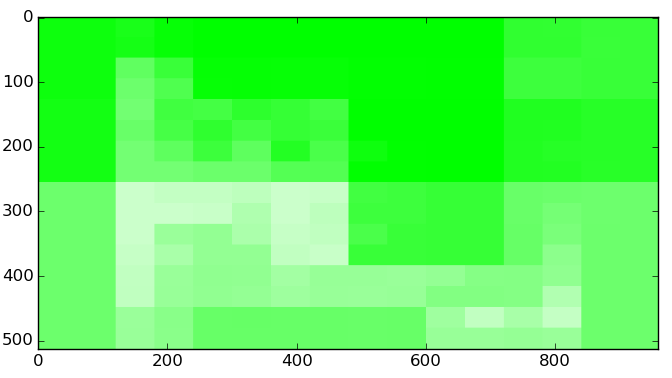
\includegraphics[keepaspectratio=true,width=\segwidth]{images/segment/401_10__animals__.png} &
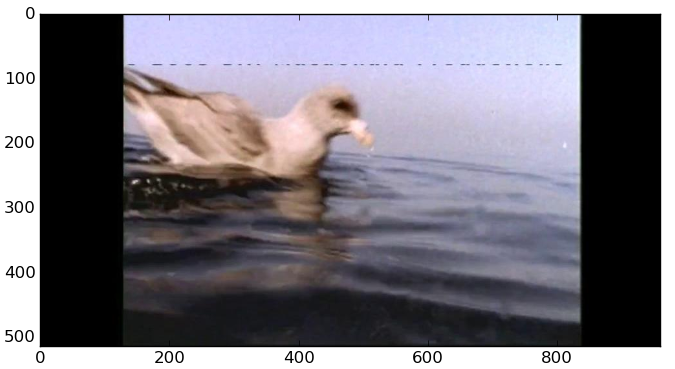
\includegraphics[keepaspectratio=true,width=\segwidth]{images/segment/401_10__image__.png} &
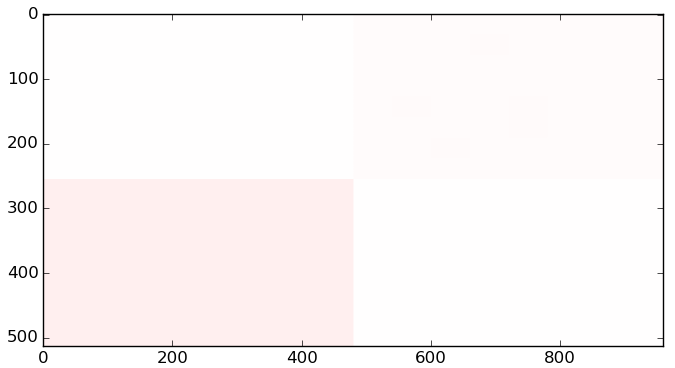
\includegraphics[keepaspectratio=true,width=\segwidth]{images/segment/401_10__plastic__.png} \\

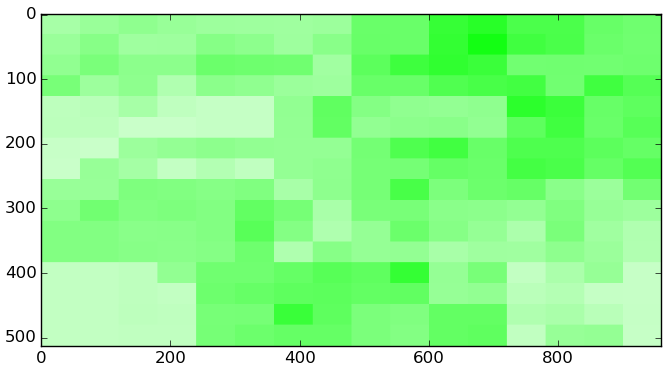
\includegraphics[keepaspectratio=true,width=\segwidth]{images/segment/701_11__animals__.png} &
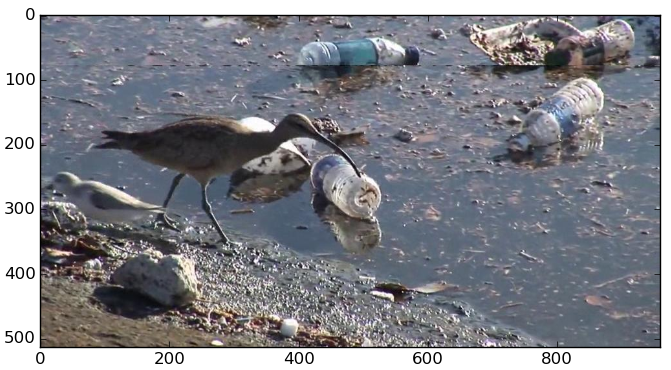
\includegraphics[keepaspectratio=true,width=\segwidth]{images/segment/701_11__image__.png} &
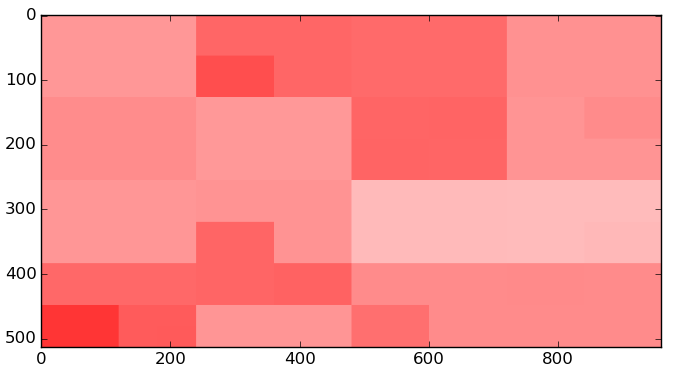
\includegraphics[keepaspectratio=true,width=\segwidth]{images/segment/701_11__plastic__.png} \\

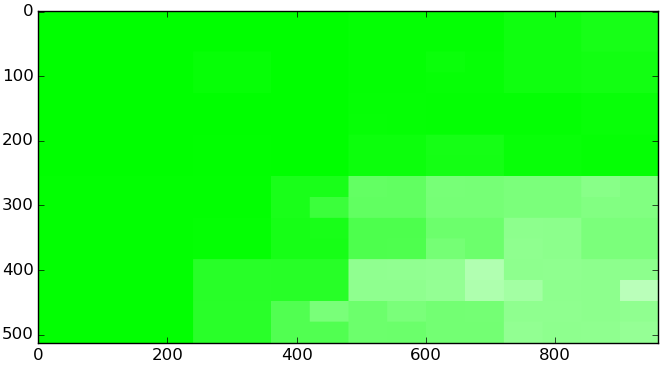
\includegraphics[keepaspectratio=true,width=\segwidth]{images/segment/2737_10__animals__.png} &
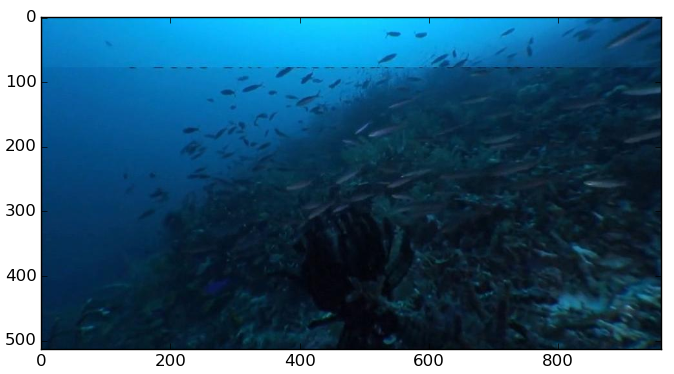
\includegraphics[keepaspectratio=true,width=\segwidth]{images/segment/2737_10__image__.png} &
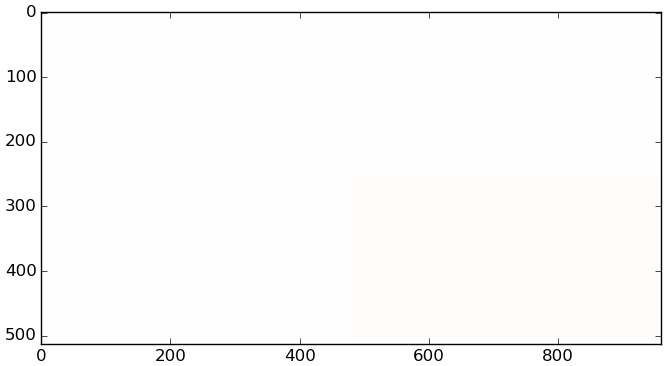
\includegraphics[keepaspectratio=true,width=\segwidth]{images/segment/2737_10__plastic__.png} \\

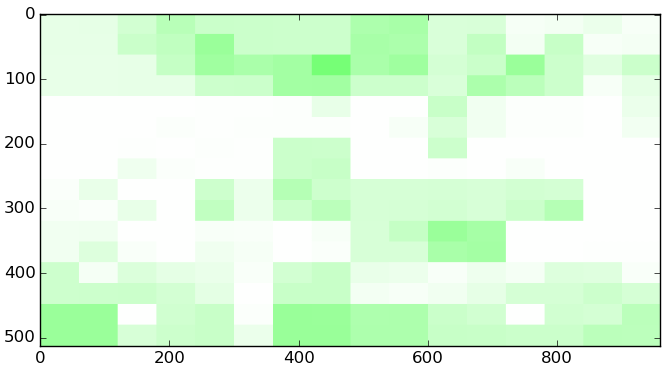
\includegraphics[keepaspectratio=true,width=\segwidth]{images/segment/4409_01__animals__.png} &
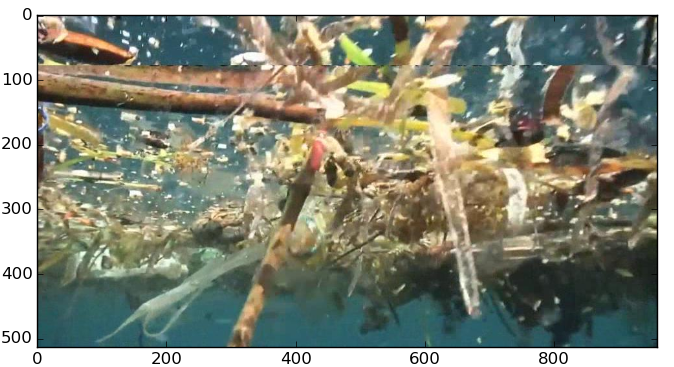
\includegraphics[keepaspectratio=true,width=\segwidth]{images/segment/4409_01__image__.png} &
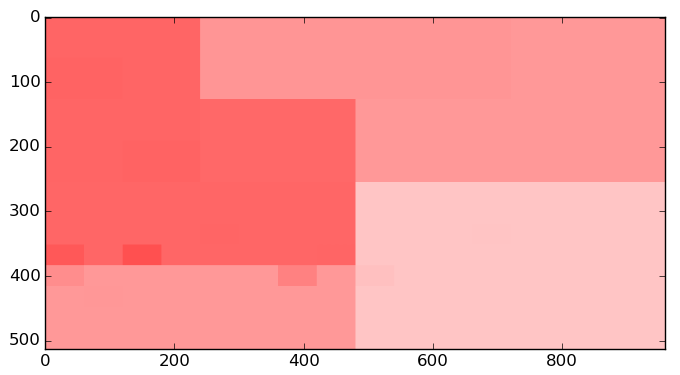
\includegraphics[keepaspectratio=true,width=\segwidth]{images/segment/4409_01__plastic__.png} \\

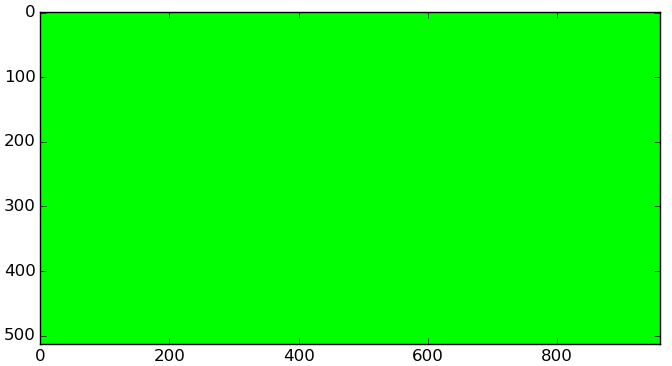
\includegraphics[keepaspectratio=true,width=\segwidth]{images/segment/5053_10__animals__.png} &
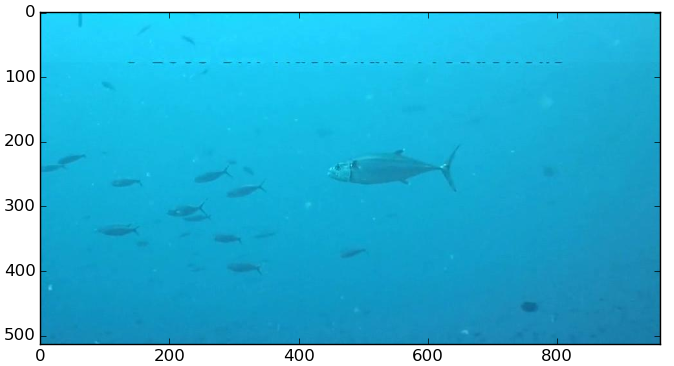
\includegraphics[keepaspectratio=true,width=\segwidth]{images/segment/5053_10__image__.png} &
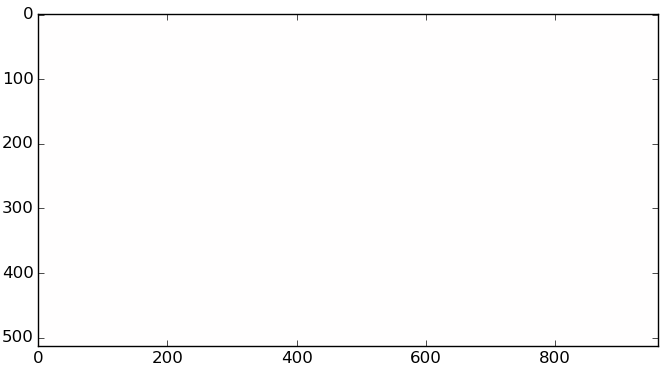
\includegraphics[keepaspectratio=true,width=\segwidth]{images/segment/5053_10__plastic__.png} \\

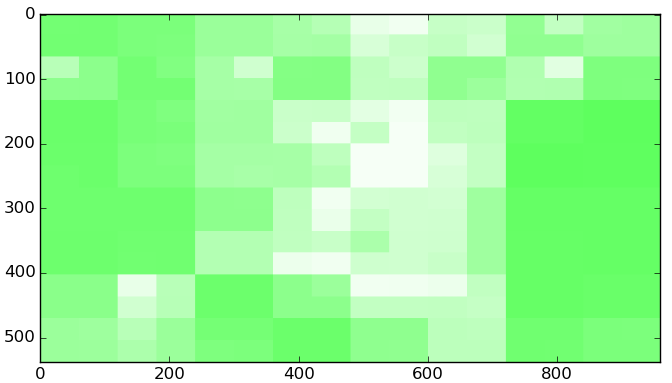
\includegraphics[keepaspectratio=true,width=\segwidth]{images/segment/20607_01__animals__.png} &
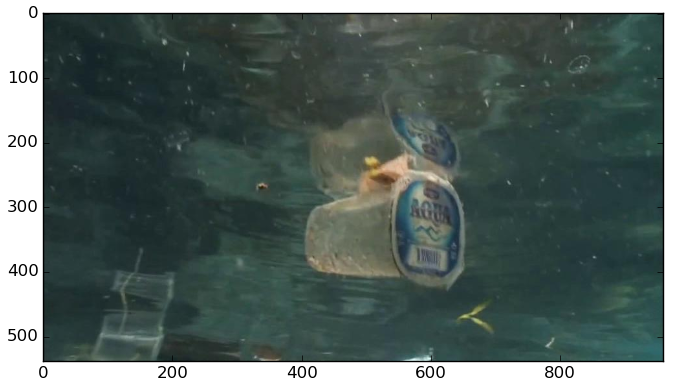
\includegraphics[keepaspectratio=true,width=\segwidth]{images/segment/20607_01__image__.png} &
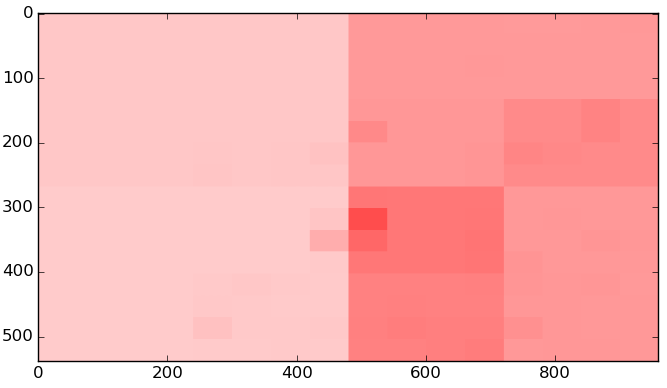
\includegraphics[keepaspectratio=true,width=\segwidth]{images/segment/20607_01__plastic__.png}
	\end{tabular}
\fi
\captionsetup{width=.8\textwidth}
\caption{Example of outcome of running an image through the segmented image pipeline. Green locates the animals and red the plastic}
\label{fig:sub-matrix}
\end{figure}
%\ifx\showpbreak\undefined \clearpage \fi

%-%\section{Conclusion}
\label{sec:Conclusion}
%Intepretatie uit resultaten
Several conclusions can be drawn from the results of this project.
%Firstly, however, no conclusion can be made from the results of the Feed Forward Network.
%The implementation used in this project did not work, nevertheless usage of a neural network for training the second-to-last layer could work.
%In the discussion I will elaborate on this.
Firstly, the Support Vector Machine has promising results.
The tests of figure \ref{fig:c14} show that the linear model has one of the highest accuracies of the different hyperplanes, while also having the smallest time to train and test.
It can therefore be concluded that a linear SVM works best for this dataset.

The test of figure \ref{fig:lin1} shows an accuracy on plastic and animal detection of less than 1\permil.
However, because the model was trained on 70\% the images in the dataset, which consists mostly of consecutive frames of short film clips, there is a substantial amount of overfitting possible.

Therefore, as shown in figure \ref{fig:lin2} another test using the complete dataset from both above and below water viewpoints, shows how the linear SVM performs on different amounts of train data.
In this case overfitting when half the dataset is used is also probable, nevertheless, the model also shows accuracy of more than 90\% when trained on merely a small part of the train-set.
Therefore it can be concluded that this method, using the second-to-last layer of a pre-trained Convolutional Neural Network on an SVM, makes it possible to detect Plastic Soup in images.

A precise conclusion from the localisation experient is difficult to draw.
The conducted test shows some results.
Several of the images show a higher confidance on locations where the consentration of plastic is higher.
However, this is not always the case; especialy with the location of marine-life.
More tests should be conducted with this technique, with possibly more annotated data, before a conclusion can be made.

Finally the usability of the promising method of using pre-trained CNNs to train on classes that were not in the original CNN is shown in this project.
Using a pre-trained CNN as a feature extractor and training another classifier is a simple technique to gain high accuracy while training on a small dataset.

%connections between existing theories and how the algorithm identifies plastic soup. including: what works? and what are the gaps?

%Figure \ref{fig:lin1} shows the improvement of accuracy when a larger train-set is used, while the enlarged train-set also increases the amount of time needed to train.
%In figures \ref{fig:c14} till \ref{fig:c14000} the increasing time needed for larger train-sets can also be seen between the figures.
%-%\ifx\showpbreak\undefined \clearpage \fi

\section{Discussion}
\label{sec:Discussion}
%intepretatie uit conclusie, beantwoord hypothese,
%\todo{kijken of subsections nodig zijn}
%====samenvatting
This project tried to contribute on solving Plastic Soup.
The amount of floating plastic in the world's oceans could be very dangerous to the environment and society \citet{moore2011plastic}.
Automating the process could help with the clean-up, therefore a system that can detect plastic was researched in this project.

A dataset was constructed for this purpose, on which a Convolutional Neural Network was used for feature extraction.
On these features a SVM classifier was trained and tested against the labels of the dataset.
As shown in section \ref{sec:Results}, the SVM had a high accuracy, even while trained on small amounts of data.

%This project tried to begin the build of autonomous agents that could clean up the ocean of plastic.
%An agent was not build, however a sizeable start was made with the vision of such an agent.
%Several state-of-the-art algorithms were used on a dataset of images containing floating plastic, animals, both or none to classify the images in one of the classes.
%One of the algorithms -- the Feed Forward Network -- trained on the second-to-last layer of a Convolutional Neural Network, did not work satisfactory.

%There are several possible reasons the Feed Forward Network used in this project did not perform well.
%Because the implementation was not part of a \texttt{Python} library, there could be bugs.
%This however does not seem probable, because the implementation was tested with a xor dataset which performed properly.

%More likely is the normalisation of the data.
%The second-to-last layer of the CNN was not normalised, while the FNN implementation used ${tanh}()$ to approximate the Sigmoid function.
%However, even a normalisation of the data did not affect the outcome.
%Bottom-line, the network was not able to learn the classes from the data.

%===interpretatie conclusie
The accurate results of the Support Vector Machine could be expected.
SVMs are known to work well in high dimensional data, as long as the amount of classes to be trained on is small.
The 4096 vector of the second-to-last layer of the CNN needed to be trained on two classes, for which both had an SVM trained on ether showing or not.

As also stated before, the high accuracy on the test set could be caused by the similarity of the frames.
Nevertheless, as high accuracy also occurs with small amounts of train-data, it is possible to conclude the system truly detects plastic in images.

The localisation however has less satisfying results.
The confidence of detecting plastic or animals does not conform consequently with what is shown on the image.
This is possibly explained by the fact that the system learned to detect plastic from a distance.
In experiments of image classification many pixels described the existence of plastic, while in these localisation experiments, a smaller amount of pixels could be used for classification.
Besides that, it is needed in the localisation to view the plastic more close-up.
Instead of detecting much plastic together, single plastic objects now need to be recognized.

%===evaluatie
%-weinig interessante dataset
%-CNN evalueren
%\todo{stukje over evaluatie onderzoek}
In this project, several aspects could have been improved for improvement of the results.
Firstly the used dataset consisted of many similar frames, which increased the chance of overfitting to this particular dataset.
Besides that, the classes that were trained on were not fairly distributed in the dataset.
An improved dataset could be used to improve the results of this project.
An improved dataset should also contain labels on parts of the images, which could improve the training and testing of the localisation of plastic within the image.

This project did not research the usage of different Convolutional Neural Networks.
A standard CNN was used to construct the feature-vector; no time was spent on researching if other networks would perform better.

Not only was assumed that the CNN worked properly that it was not further tested, also the parameters with which the SVM was tested were not statistical analysed; no cross-fold validation was conducted.

%===vervolgonderzoek
%-localisatie verbeteren mbv BING oid
%\todo{stukje over vervolgonderzoek, oa verbeteren plastic-herkenning (ook locatie) en maken van autonomous agent voor schepen}

Obviously, further research in this domain could correct the mistakes made in this project.
A better dataset and more cross-validation could improve the localisation of detecting plastic.
Even so, training the system to recognise plastic on several scales could increase the performance on localisation.

Other manners to improve the localisation of the plastic within the images, are the use of other algorithms.
If more complex algorithms are used for object detection in the image, the blobs resulting from those could be input for the pipeline, instead of the now used segmentation-pyramid.
One of the algorithms that could be used for this is BING \citeneed; this project did not have the time to implement one of these algorithms.

Before the system proposed in this project could be used for real-world applications, more research is needed.
However, this project showed the possibility of using state-of-the-art Computer Vision techniques to detect Plastic Soup.
More research building on the results of this project could result in applications that can detect Plastic Soup.

%===afsluiting
This project is one of the many recent projects that show the possibilities of Convolutional Neural Networks.
Besides that, it also shows how the Artificial Intelligence can be used to help solving environmental problems.
I do not think the hippie movement in the '60s could imagine that AI could solve their problems for them today.

%\subsection{Future research}
%Evatuatie onderzoek, vervolgonderzoek


%\ifx\showpbreak\undefined \clearpage \fi

\vfill
\bibliographystyle{abbrvnat}
\bibliography{Tex_sources/bib}

\clearpage

\ifx\showapp\undefined
\begin{appendix}
\renewcommand{\thesubsection}{\thesection.\roman{subsection}}
\renewcommand{\thesubsubsection}{\thesubsection - \arabic{subsubsection}}
\addtocontents{toc}{\setcounter{tocdepth}{2}}

\section{\texttt{Python} code of the project}
\label{sec:ap-code}

\section{Output of \texttt{Python} code}
\label{sec:ap-out}

\subsection{SVM}
\begin{tabular}{ p{0.2\textwidth } | p{0.8\textwidth } }
abbrivation & meaning \\ \hline
type & which type of model used for the fitting hyperplane; poly mean polynomial, where the last digit stands for the degree; rbf is gaussian, where the last digit stands for gamma \\
Ttrain & the amount of time in seconds the complete training took \\
Ttest & the amount of time in seconds the complete testing took \\
Dsize & the amount of data-points used for training the model \\
Vsize & the amount of data-points used for testing the model \\
Bco & the amount of test-points that were correct\footnote{correct means here having the same output as the label, so both \texttt{11} and \texttt{00} are considered correct i.e. an iff} on both classes \\
Pco & the amount of test-points that were correct only on the plastic class \\
Aco & the amount of test-points that were correct only on the animal class \\
Bac & the accuracy on both classes i.e. $\frac{Bco}{Vsize}$ \\
Pac & the accuracy on the plastic class i.e. $\frac{Bco+Pco}{Vsize}$ \\
Aac & the accuracy on the animals class i.e. $\frac{Bco+Aco}{Vsize}$
\end{tabular}
{\small
\begin{longtable}{r|r|r|r|r|r|r|r|r|r|r|r}
\subsubsection{Train and validate below water}
\begin{longtable}{r|r|r|r|r|r|r|r|r|r|r|r}
          type &  Ttrain &   Ttest & Dsize & Vsize &   Bco &   Pco &   Aco &   Bfa &   Bac &   Pac &   Aac \\
   poly,1.0,2  &     0.0 &     0.7 &    14 &  2061 &  1144 &   378 &   453 &    86 & 0.555 & 0.738 & 0.775 \\
   poly,1.0,3  &     0.0 &     1.0 &    14 &  2061 &  1099 &   410 &   497 &    55 & 0.533 & 0.732 & 0.774 \\
   poly,1.0,4  &     0.0 &     1.0 &    14 &  2061 &   890 &   593 &   536 &    42 & 0.432 & 0.720 & 0.692 \\
   poly,1.0,5  &     0.0 &     0.8 &    14 &  2061 &   779 &   698 &   548 &    36 & 0.378 & 0.717 & 0.644 \\
   poly,1.0,6  &     0.0 &     1.2 &    14 &  2061 &   988 &   489 &   539 &    45 & 0.479 & 0.717 & 0.741 \\
   poly,1.0,7  &     0.0 &     0.9 &    14 &  2061 &  1237 &   235 &   352 &   237 & 0.600 & 0.714 & 0.771 \\
   poly,1.0,8  &     0.0 &     1.2 &    14 &  2061 &  1216 &   252 &   204 &   389 & 0.590 & 0.712 & 0.689 \\
   poly,1.0,9  &     0.0 &     1.1 &    14 &  2061 &  1214 &   251 &   108 &   488 & 0.589 & 0.711 & 0.641 \\
  rbf,1.0,0.0  &     0.0 &     0.9 &    14 &  2061 &  1174 &   271 &    47 &   569 & 0.570 & 0.701 & 0.592 \\
  rbf,1.0,0.1  &     0.0 &     0.8 &    14 &  2061 &  1174 &   271 &    47 &   569 & 0.570 & 0.701 & 0.592 \\
  rbf,1.0,0.2  &     0.0 &     1.2 &    14 &  2061 &  1174 &   271 &    47 &   569 & 0.570 & 0.701 & 0.592 \\
  rbf,1.0,0.3  &     0.0 &     1.2 &    14 &  2061 &   392 &  1053 &   594 &    22 & 0.190 & 0.701 & 0.478 \\
  rbf,1.0,0.4  &     0.0 &     1.0 &    14 &  2061 &   354 &  1091 &   594 &    22 & 0.172 & 0.701 & 0.460 \\
  rbf,1.0,0.5  &     0.0 &     1.2 &    14 &  2061 &   338 &  1107 &   594 &    22 & 0.164 & 0.701 & 0.452 \\
  rbf,1.0,0.6  &     0.0 &     0.8 &    14 &  2061 &   330 &  1115 &   594 &    22 & 0.160 & 0.701 & 0.448 \\
  rbf,1.0,0.7  &     0.0 &     0.8 &    14 &  2061 &   325 &  1120 &   594 &    22 & 0.158 & 0.701 & 0.446 \\
  rbf,1.0,0.8  &     0.0 &     1.2 &    14 &  2061 &   317 &  1128 &   594 &    22 & 0.154 & 0.701 & 0.442 \\
  rbf,1.0,0.9  &     0.0 &     0.7 &    14 &  2061 &   316 &  1129 &   594 &    22 & 0.153 & 0.701 & 0.442 \\
  rbf,1.0,1.0  &     0.0 &     0.7 &    14 &  2061 &   316 &  1129 &   594 &    22 & 0.153 & 0.701 & 0.442 \\
   linear,1.0  &     0.0 &     0.6 &    14 &  2061 &  1177 &   350 &   401 &   133 & 0.571 & 0.741 & 0.766 \\
          type &  Ttrain &   Ttest & Dsize & Vsize &   Bco &   Pco &   Aco &   Bfa &   Bac &   Pac &   Aac \\
   poly,1.0,2  &     0.4 &     4.5 &   140 &  2061 &  1890 &    71 &    45 &    55 & 0.917 & 0.951 & 0.939 \\
   poly,1.0,3  &     0.5 &     5.6 &   140 &  2061 &  1876 &    77 &    50 &    58 & 0.910 & 0.948 & 0.934 \\
   poly,1.0,4  &     0.4 &     6.3 &   140 &  2061 &  1847 &    91 &    56 &    67 & 0.896 & 0.940 & 0.923 \\
   poly,1.0,5  &     0.4 &     7.1 &   140 &  2061 &  1820 &   105 &    68 &    68 & 0.883 & 0.934 & 0.916 \\
   poly,1.0,6  &     0.6 &     7.5 &   140 &  2061 &  1789 &   114 &    76 &    82 & 0.868 & 0.923 & 0.905 \\
   poly,1.0,7  &     0.6 &     7.7 &   140 &  2061 &  1759 &   123 &    85 &    94 & 0.853 & 0.913 & 0.895 \\
   poly,1.0,8  &     0.4 &     7.6 &   140 &  2061 &  1733 &   133 &    78 &   117 & 0.841 & 0.905 & 0.879 \\
   poly,1.0,9  &     0.6 &     8.3 &   140 &  2061 &  1713 &   143 &    75 &   130 & 0.831 & 0.901 & 0.868 \\
  rbf,1.0,0.0  &     0.4 &     7.2 &   140 &  2061 &  1235 &   253 &    89 &   484 & 0.599 & 0.722 & 0.642 \\
  rbf,1.0,0.1  &     0.4 &     7.2 &   140 &  2061 &  1140 &   305 &    23 &   593 & 0.553 & 0.701 & 0.564 \\
  rbf,1.0,0.2  &     0.6 &    10.3 &   140 &  2061 &  1140 &   305 &    23 &   593 & 0.553 & 0.701 & 0.564 \\
  rbf,1.0,0.3  &     0.6 &    10.1 &   140 &  2061 &  1140 &   305 &    22 &   594 & 0.553 & 0.701 & 0.564 \\
  rbf,1.0,0.4  &     0.6 &     9.5 &   140 &  2061 &  1140 &   305 &    22 &   594 & 0.553 & 0.701 & 0.564 \\
  rbf,1.0,0.5  &     0.6 &    10.4 &   140 &  2061 &  1140 &   305 &    22 &   594 & 0.553 & 0.701 & 0.564 \\
  rbf,1.0,0.6  &     0.4 &     7.8 &   140 &  2061 &  1140 &   305 &    22 &   594 & 0.553 & 0.701 & 0.564 \\
  rbf,1.0,0.7  &     0.4 &     7.1 &   140 &  2061 &  1140 &   305 &    22 &   594 & 0.553 & 0.701 & 0.564 \\
  rbf,1.0,0.8  &     0.6 &    10.4 &   140 &  2061 &  1140 &   305 &    22 &   594 & 0.553 & 0.701 & 0.564 \\
  rbf,1.0,0.9  &     0.4 &     6.4 &   140 &  2061 &  1140 &   305 &    22 &   594 & 0.553 & 0.701 & 0.564 \\
  rbf,1.0,1.0  &     0.4 &     6.8 &   140 &  2061 &  1140 &   305 &    22 &   594 & 0.553 & 0.701 & 0.564 \\
   linear,1.0  &     0.2 &     3.1 &   140 &  2061 &  1851 &   101 &    54 &    55 & 0.898 & 0.947 & 0.924 \\
          type &  Ttrain &   Ttest & Dsize & Vsize &   Bco &   Pco &   Aco &   Bfa &   Bac &   Pac &   Aac \\
   poly,1.0,2  &    10.1 &    17.2 &  1400 &  2061 &  2048 &     8 &     5 &     0 & 0.994 & 0.998 & 0.996 \\
   poly,1.0,3  &    14.1 &    20.5 &  1400 &  2061 &  2049 &     7 &     5 &     0 & 0.994 & 0.998 & 0.997 \\
   poly,1.0,4  &    13.0 &    17.1 &  1400 &  2061 &  2047 &     9 &     5 &     0 & 0.993 & 0.998 & 0.996 \\
   poly,1.0,5  &    12.7 &    18.8 &  1400 &  2061 &  2044 &    11 &     6 &     0 & 0.992 & 0.997 & 0.995 \\
   poly,1.0,6  &    20.6 &    30.3 &  1400 &  2061 &  2042 &    13 &     6 &     0 & 0.991 & 0.997 & 0.994 \\
   poly,1.0,7  &    22.8 &    32.9 &  1400 &  2061 &  2032 &    18 &    11 &     0 & 0.986 & 0.995 & 0.991 \\
   poly,1.0,8  &    16.1 &    23.3 &  1400 &  2061 &  2024 &    21 &    11 &     5 & 0.982 & 0.992 & 0.987 \\
   poly,1.0,9  &    23.2 &    38.5 &  1400 &  2061 &  2013 &    23 &    15 &    10 & 0.977 & 0.988 & 0.984 \\
  rbf,1.0,0.0  &    29.8 &    40.6 &  1400 &  2061 &  2040 &    10 &    11 &     0 & 0.990 & 0.995 & 0.995 \\
  rbf,1.0,0.1  &    64.7 &    93.2 &  1400 &  2061 &  1140 &   305 &    38 &   578 & 0.553 & 0.701 & 0.572 \\
  rbf,1.0,0.2  &    58.7 &    77.5 &  1400 &  2061 &  1140 &   305 &    24 &   592 & 0.553 & 0.701 & 0.565 \\
  rbf,1.0,0.3  &    57.6 &    79.9 &  1400 &  2061 &  1140 &   305 &    22 &   594 & 0.553 & 0.701 & 0.564 \\
  rbf,1.0,0.4  &    58.6 &    82.3 &  1400 &  2061 &  1140 &   305 &    22 &   594 & 0.553 & 0.701 & 0.564 \\
  rbf,1.0,0.5  &    58.2 &    82.1 &  1400 &  2061 &  1140 &   305 &    22 &   594 & 0.553 & 0.701 & 0.564 \\
  rbf,1.0,0.6  &    51.7 &    91.9 &  1400 &  2061 &  1140 &   305 &    22 &   594 & 0.553 & 0.701 & 0.564 \\
  rbf,1.0,0.7  &    50.9 &    83.2 &  1400 &  2061 &  1140 &   305 &    22 &   594 & 0.553 & 0.701 & 0.564 \\
  rbf,1.0,0.8  &    48.9 &    87.9 &  1400 &  2061 &  1140 &   305 &    22 &   594 & 0.553 & 0.701 & 0.564 \\
  rbf,1.0,0.9  &    54.5 &    45.1 &  1400 &  2061 &  1140 &   305 &    22 &   594 & 0.553 & 0.701 & 0.564 \\
  rbf,1.0,1.0  &    54.2 &    78.5 &  1400 &  2061 &  1140 &   305 &    22 &   594 & 0.553 & 0.701 & 0.564 \\
   linear,1.0  &     5.6 &     8.3 &  1400 &  2061 &  2047 &     6 &     8 &     0 & 0.993 & 0.996 & 0.997 \\
          type &  Ttrain &   Ttest & Dsize & Vsize &   Bco &   Pco &   Aco &   Bfa &   Bac &   Pac &   Aac \\
   poly,1.0,2  &  1124.4 &   155.7 & 14000 &  2061 &  2015 &    24 &    22 &     0 & 0.978 & 0.989 & 0.988 \\
   poly,1.0,3  &  2068.0 &   277.0 & 14000 &  2061 &  1987 &    47 &    23 &     4 & 0.964 & 0.987 & 0.975 \\
   poly,1.0,4  &  3331.6 &   459.8 & 14000 &  2061 &  1777 &   162 &    84 &    38 & 0.862 & 0.941 & 0.903 \\
   poly,1.0,5  &  4678.5 &   646.8 & 14000 &  2061 &  1527 &   231 &    87 &   216 & 0.741 & 0.853 & 0.783 \\
   poly,1.0,6  &  5198.9 &   696.6 & 14000 &  2061 &  1249 &   278 &    55 &   479 & 0.606 & 0.741 & 0.633 \\
   poly,1.0,7  &  5282.2 &   706.6 & 14000 &  2061 &  1192 &   305 &    22 &   542 & 0.578 & 0.726 & 0.589 \\
   poly,1.0,8  &  5193.3 &   719.4 & 14000 &  2061 &  1173 &   305 &    24 &   559 & 0.569 & 0.717 & 0.581 \\
   poly,1.0,9  &  5083.9 &   714.2 & 14000 &  2061 &  1157 &   305 &    22 &   577 & 0.561 & 0.709 & 0.572 \\
  rbf,1.0,0.0  &   586.3 &    86.2 & 14000 &  2061 &  2043 &     6 &    12 &     0 & 0.991 & 0.994 & 0.997 \\
  rbf,1.0,0.1  & 24560.3 &  1067.4 & 14000 &  2061 &  1230 &   285 &   130 &   416 & 0.597 & 0.735 & 0.660 \\
  rbf,1.0,0.2  & 25139.6 &  1069.5 & 14000 &  2061 &  1152 &   304 &    57 &   548 & 0.559 & 0.706 & 0.587 \\
  rbf,1.0,0.3  & 25104.7 &  1059.1 & 14000 &  2061 &  1142 &   305 &    31 &   583 & 0.554 & 0.702 & 0.569 \\
  rbf,1.0,0.4  & 25389.9 &  1052.6 & 14000 &  2061 &  1142 &   305 &    26 &   588 & 0.554 & 0.702 & 0.567 \\
  rbf,1.0,0.5  & 24877.4 &  1055.4 & 14000 &  2061 &  1142 &   305 &    21 &   593 & 0.554 & 0.702 & 0.564 \\
  rbf,1.0,0.6  & 26216.1 &  1062.9 & 14000 &  2061 &  1142 &   305 &    20 &   594 & 0.554 & 0.702 & 0.564 \\
  rbf,1.0,0.7  & 25266.2 &   618.3 & 14000 &  2061 &  1142 &   305 &    20 &   594 & 0.554 & 0.702 & 0.564 \\
  rbf,1.0,0.8  & 26166.7 &  1072.2 & 14000 &  2061 &  1141 &   305 &    21 &   594 & 0.554 & 0.702 & 0.564 \\
  rbf,1.0,0.9  & 18654.6 &   607.0 & 14000 &  2061 &  1141 &   305 &    21 &   594 & 0.554 & 0.702 & 0.564 \\
  rbf,1.0,1.0  & 16250.9 &   399.1 & 14000 &  2061 &  1140 &   305 &    22 &   594 & 0.553 & 0.701 & 0.564 \\
   linear,1.0  &    74.6 &     8.4 & 14000 &  2061 &  2058 &     2 &     1 &     0 & 0.999 & 1.000 & 0.999 \\
\end{longtable}
\subsubsection{Train and test below water}
\begin{longtable}{r|r|r|r|r|r|r|r|r|r|r|r}
    type &  Ttrain &   Ttest & Dsize & Vsize &   Bco &   Pco &   Aco &   Bfa &   Bac &   Pac &   Aac \\
    linear,1.0 &     0.0 &     5.9 &     9 &  4123 &  2228 &   797 &   748 &   350 & 0.540 & 0.734 & 0.722 \\
    linear,1.0 &     0.0 &     7.8 &    18 &  4123 &  2402 &   726 &   795 &   200 & 0.583 & 0.759 & 0.775 \\
    linear,1.0 &     0.4 &    14.5 &    90 &  4123 &  3534 &   215 &   213 &   161 & 0.857 & 0.909 & 0.909 \\
    linear,1.0 &     0.8 &    19.6 &   180 &  4123 &  3753 &   136 &   148 &    86 & 0.910 & 0.943 & 0.946 \\
    linear,1.0 &    10.0 &    27.5 &   900 &  4123 &  4057 &    25 &    32 &     9 & 0.984 & 0.990 & 0.992 \\
    linear,1.0 &    21.1 &    29.1 &  1800 &  4123 &  4092 &    13 &    15 &     3 & 0.992 & 0.996 & 0.996 \\
    linear,1.0 &    82.5 &    23.2 &  9000 &  4123 &  4118 &     3 &     2 &     0 & 0.999 & 1.000 & 0.999 \\
    linear,1.0 &   123.8 &    16.8 & 18000 &  4123 &  4119 &     2 &     2 &     0 & 0.999 & 1.000 & 1.000 \\
\end{longtable}
\ifx\showmixi\undefined
\subsubsection{Train on below water, test on above water}
\begin{longtable}{r|r|r|r|r|r|r|r|r|r|r|r}
          type &  Ttrain &   Ttest & Dsize & Vsize &   Bco &   Pco &   Aco &   Bfa &   Bac &   Pac &   Aac \\
    linear,1.0 &     0.0 &     4.4 &     9 &  3311 &  1396 &  1530 &    97 &   288 & 0.422 & 0.884 & 0.451 \\
    linear,1.0 &     0.0 &     6.8 &    18 &  3311 &  1578 &  1348 &   173 &   212 & 0.477 & 0.884 & 0.529 \\
    linear,1.0 &     0.4 &    12.6 &    90 &  3311 &  1673 &  1208 &   167 &   263 & 0.505 & 0.870 & 0.556 \\
    linear,1.0 &     0.6 &    15.5 &   180 &  3311 &  1615 &  1090 &   339 &   267 & 0.488 & 0.817 & 0.590 \\
    linear,1.0 &     9.8 &    21.7 &   900 &  3311 &  1684 &   999 &   277 &   351 & 0.509 & 0.810 & 0.592 \\
    linear,1.0 &    20.7 &    23.1 &  1800 &  3311 &  1757 &  1042 &   242 &   270 & 0.531 & 0.845 & 0.604 \\
    linear,1.0 &    79.0 &    18.7 &  9000 &  3311 &  1659 &  1301 &   248 &   103 & 0.501 & 0.894 & 0.576 \\
    linear,1.0 &   118.4 &    13.5 & 18000 &  3311 &  1685 &  1272 &   237 &   117 & 0.509 & 0.893 & 0.580 
\end{longtable}
\subsubsection{Train on above water, test on below water}
\begin{longtable}{r|r|r|r|r|r|r|r|r|r|r|r}
          type &  Ttrain &   Ttest & Dsize & Vsize &   Bco &   Pco &   Aco &   Bfa &   Bac &   Pac &   Aac \\
    linear,1.0 &     0.0 &     5.9 &     9 &  4123 &  2147 &   771 &   282 &   923 & 0.521 & 0.708 & 0.589 \\
    linear,1.0 &     0.0 &     7.6 &    18 &  4123 &  2218 &   731 &   171 &  1003 & 0.538 & 0.715 & 0.579 \\
    linear,1.0 &     0.4 &    14.5 &    90 &  4123 &  1724 &   909 &   482 &  1008 & 0.418 & 0.639 & 0.535 \\
    linear,1.0 &     0.6 &    17.0 &   180 &  4123 &  1660 &  1073 &   573 &   817 & 0.403 & 0.663 & 0.542 \\
    linear,1.0 &     6.6 &    20.6 &   900 &  4123 &  1735 &   954 &   413 &  1021 & 0.421 & 0.652 & 0.521 \\
    linear,1.0 &    13.5 &    18.2 &  1800 &  4123 &  1894 &   872 &   378 &   979 & 0.459 & 0.671 & 0.551 \\
    linear,1.0 &    46.2 &    12.4 &  9000 &  4123 &  1885 &  1041 &   284 &   913 & 0.457 & 0.710 & 0.526 \\
    linear,1.0 &    55.9 &     9.9 & 18000 &  4123 &  1851 &   975 &   375 &   922 & 0.449 & 0.685 & 0.540 
\end{longtable}
\fi

\subsubsection{Train and test mixed dataset}
\begin{longtable}{r|r|r|r|r|r|r|r|r|r|r|r}
          type &  Ttrain &   Ttest & Dsize & Vsize &   Bco &   Pco &   Aco &   Bfa &   Bac &   Pac &   Aac \\
   linear,1.0  &     0.0 &    17.0 &     9 & 18583 & 11538 &  2972 &   846 &  3227 & 0.621 & 0.781 & 0.666 \\
   linear,1.0  &     0.0 &    33.1 &    18 & 18583 & 10853 &  3951 &  2316 &  1463 & 0.584 & 0.797 & 0.709 \\
   linear,1.0  &     0.3 &    77.8 &    90 & 18583 & 15465 &  1336 &  1308 &   474 & 0.832 & 0.904 & 0.903 \\
   linear,1.0  &     1.4 &    95.4 &   180 & 18583 & 16713 &   827 &   686 &   357 & 0.899 & 0.944 & 0.936 \\
   linear,1.0  &    12.1 &   169.0 &   900 & 18583 & 18134 &   243 &   196 &    10 & 0.976 & 0.989 & 0.986 \\
   linear,1.0  &    31.5 &   186.6 &  1800 & 18583 & 18325 &   139 &   112 &     7 & 0.986 & 0.994 & 0.992 \\
   linear,1.0  &   169.7 &   149.2 &  9000 & 18583 & 18544 &    24 &    14 &     1 & 0.998 & 0.999 & 0.999 \\
   linear,1.0  &   293.2 &   113.2 & 18000 & 18583 & 18568 &     7 &     7 &     1 & 0.999 & 1.000 & 1.000 \\
\end{longtable}
\end{longtable}
}

\end{appendix}
\fi
\end{document}
